\journalappendix{Readout Estimates and Temporal Support}{app:readout}

Table~\ref{tab:readout-detail} supplies the complete present-state contrasts behind Figure~\ref{fig:readout}.
%
Sentence counts differ because each model generates its own solution and contributes its own labelled sentences.
%
The independent question and family population is common.
%
Positive RIG favors the routing-augmented classifier.
%

% Adapted from SPSD tab:main-results and SYNCO tab:mainRes.
\begin{table}[hb]
\centering\small
\caption{Routing information gain (RIG): text-baseline cross-entropy minus routing-augmented cross-entropy (nats per sentence), with 95\% confidence intervals as subscripts.
%
Each evaluated model uses 522 questions in 509 families.
%
Intervals retain the original model-specific seven-comparison family-bootstrap correction.
%
Bold and underline mark the largest and second-largest mean gains descriptively.
%
Dashes denote pending LFM2.5 results.}
\label{tab:readout-detail}
\setlength{\tabcolsep}{2.5pt}
\begin{adjustbox}{max width=\linewidth}
\begin{tabular}{@{}lrc@{}}
\toprule
Model & Sentences & RIG (nats) $\uparrow$ \\
\midrule
\modelname{openai}{GPT-OSS-20B} & 37,549 & \cid{0.07858}{0.01679}{0.01709} \\ 
\modelname{nvidia}{\shortstack[l]{Nemotron-3.5-Lightning\\30B-A3B}} & 35,334 & \cid{0.13721}{0.01902}{0.01907} \\ 
\modelname{qwen}{Qwen3.5-35B-A3B} & 34,740 & \secondcid{0.14090}{0.01309}{0.01269} \\ 
\modelname{qwen}{Qwen3.6-35B-A3B} & 35,484 & \cid{0.13899}{0.01297}{0.01378} \\ 
\modelname{gemma}{Gemma-4-26B-A4B} & 31,902 & \bestcid{0.14866}{0.01174}{0.01269} \\ 
\modelname{zhipu}{GLM-4.7-Flash (30B-A3B)} & 38,931 & \cid{0.13679}{0.01644}{0.01623} \\ 
\modelname{qwen}{Qwen3-30B-A3B} & 36,445 & \cid{0.09427}{0.01326}{0.01502} \\ 
\modelname{liquid}{LFM2.5-24B-A2B} & \textemdash & \textemdash \\
\bottomrule
\end{tabular}
\end{adjustbox}
\end{table}


\subsection{Readout representations and model selection}
\label{app:readout-features}

The readout tests information about the assigned sentence label while holding the evaluation families fixed.
%
Token-identity features use 4,096 buckets, retain terms supported by at least two training sentences, and apply sublinear term-frequency/inverse-document-frequency weighting.
%
Each resulting row is normalized to Euclidean length one and scaled by ten.
%
The extended reader-context representation hashes word unigrams and bigrams and character 3-, 4-, and 5-grams into $2^{18}$ buckets, with the same row scale.
%
Only training data determine the frequency weights.
%
Dense routing features are standardized within the training fold.
%
Coordinate means and population standard deviations use the training rows.
%
A nonfinite mean is replaced by zero, a standard deviation at most $10^{-12}$ by one, and a missing standardized value by zero.
%

Let $a_{\ell,t}$ be the top-1 expert at sparse layer $\ell$ for token $t$.
%
For each adjacent layer pair, training-token counts $N_\ell(a,b)$ define the smoothed conditional probability
\begin{equation}
\widehat p_\ell(b\mid a)=
\frac{N_\ell(a,b)+0.5}{\sum_{b'}N_\ell(a,b')+0.5E}.
\end{equation}
Here $E$ is the number of experts per sparse layer.
%
Depth-path surprise $D_s$ is the sentence mean of $-\log\widehat p_\ell(a_{\ell+1,t}\mid a_{\ell,t})$, averaged equally over its tokens and the $L-1$ adjacent layer pairs.
%
It measures how unexpected the observed sequence of expert identities across depth is under the training transitions.
%
It is nonnegative in nats and has no population-independent finite upper bound.
%

Temporal persistence measures the fraction of layers retaining the same top-1 expert between consecutive tokens.
%
For a sentence $j$, let $A_j$ contain its token positions whose preceding token is adjacent and belongs to that sentence.
%
The feature is
\begin{equation}
R_j=\frac{1}{|A_j|L}\sum_{t\in A_j}\sum_{\ell=1}^{L}
\mathbf{1}\{a_{\ell,t}=a_{\ell,t-1}\}.
\end{equation}
Its range is zero to one, where one means that every layer retains its top-1 identity across every supported token pair.
%
When $A_j$ is empty, the feature is missing and becomes zero after training-fold standardization, the standardized training mean.
%
Neither feature bridges a sentence boundary or a missing-token gap.
%

The routing composition is centered on the training mean and projected to 64 principal components.
%
The retained randomized decomposition uses 16 oversampling directions and four power iterations.
%
Routing features also contain depth-path surprise and temporal persistence.
%
Multinomial ridge fitting selects its penalty from $10^{-3},10^{-2},10^{-1},1,10,100$ by inner held-out cross-entropy, breaking ties toward stronger regularization.
%
The five outer and three inner folds keep duplicate families together.
%
All transforms are fitted anew on each training split.
%
The saved intervals condition on these fitted readouts.
%
The routing-augmented penalty is 0.01 in every outer fold for the seven original models and 0.001 for LFM2.5.
%
The text penalty is 0.001 throughout for GPT-OSS, Nemotron, Qwen3.5, Qwen3.6 and Qwen3-30B, and 0.01 throughout for Gemma.
%
GLM uses 0.001, 0.01, 0.01, 0.001 and 0.001 in fold order.
%

\subsection{Next-state support}
\label{app:next-state}
The original next-state endpoint and its source-length sensitivity have different question and pair counts (Table~\ref{tab:next-state}).
%
Both use only tokens owned by the source sentence.
%
The sensitivity retains sources with at least 32 tokens, ensuring a full 16-token trailing window.
%
It restricts eligible pairs without restricting the sentences used to build profiles within the selected training attempts.
%
Loss averages pairs within a question before averaging questions, and resampling keeps duplicate families together.
%

% Adapted from SPSD tab:main-results and SYNCO tab:mainRes.
\begin{table}[htb]
\centering\small
\caption{Anticipatory routing gain (ARG): past-text/history baseline cross-entropy minus routing-augmented cross-entropy (nats per adjacent pair), with 95\% confidence intervals as subscripts.
%
Intervals retain the original six-comparison family-bootstrap correction.
%
Bold and underline mark the larger and second-largest mean gains within each source-length condition.
%
The length column gives the minimum source-sentence length in tokens.
%
Both use source-owned tokens.}
\label{tab:next-state}
\setlength{\tabcolsep}{2.5pt}
\begin{adjustbox}{max width=\linewidth}
\begin{tabular}{@{}llrrc@{}}
\toprule
Model & Length & Questions & Pairs & ARG (nats) $\uparrow$ \\
\midrule
\modelname{openai}{GPT-OSS-20B} & None & 509 & 10,209 & \secondcid{0.02073}{0.00472}{0.00475} \\ 
\modelname{openai}{GPT-OSS-20B} & 32 & 308 & 797 & \secondcid{0.01570}{0.00923}{0.01005} \\ 
\modelname{qwen}{Qwen3.6-35B-A3B} & None & 494 & 2,492 & \bestcid{0.05570}{0.01417}{0.01374} \\ 
\modelname{qwen}{Qwen3.6-35B-A3B} & 32 & 160 & 213 & \bestcid{0.03438}{0.01427}{0.01489} \\ 
\bottomrule
\end{tabular}
\end{adjustbox}
\end{table}


The next-state profiles use all available labelled sentences from the training attempts represented in a fold.
%
Each sentence contributes its whole-sentence selected-slot histogram.
%
The raw marginal $\bar\pi^0$ averages these histograms within attempts, then across attempts.
%
For class $c$, $\widehat\pi^c$ first averages sentences of that class within an attempt, then averages the supported attempts.
%
Let $n_c$ be the number of training sentences assigned to $c$.
%
The regularized profiles are
\begin{equation}
 \pi^0=F_\epsilon(\bar\pi^0),\qquad
 \pi^c=F_\epsilon\!\left(
 \frac{n_c\widehat\pi^c+50\bar\pi^0}{n_c+50}\right),
\label{eq:routing-profiles}
\end{equation}
where $F_\epsilon$ floors each entry at $\epsilon=10^{-6}$ and then normalizes across experts within each layer.
%
An unsupported class uses the marginal profile.
%
The seven scores in Equation~\ref{eq:next-features} are standardized on the training rows before fitting the readout.
%

The sensitivity uses a restricted source-length population and is not an independent replication.
%
Six models have no completed next-state estimate.

% Necessary local flush: the next-state table belongs to Appendix A.2.
\FloatBarrier
\journalappendix{Expert Retention by Family Fold}{app:selection}

Table~\ref{tab:selection-folds} retains every model, fold, and selection method from the 75\%-retention comparison.
%
Each model uses the same five assignments of duplicate families.
%
A held-out family contributes to one test fold, while the four remaining folds provide training data.
%
Class balancing and frequency share the same labelled inputs, quotas, and tie rule.
%
The random priorities are fixed per model.
%

% Multipage longtable: retained outside adjustbox so page breaks remain available.
% Compact 2pt intercolumn spacing fits the full model identities without text scaling.
% Adapted from SPSD tab:main-results and SYNCO tab:mainRes.
\begingroup\small
\setlength{\tabcolsep}{2pt}
\begin{longtable}{lrrrrr}
\caption{Per-fold weakest-state coverage (WSC) of native selected slots (\%) at 75\% retention.
%
These are diagnostic fold estimates, without estimated confidence intervals: test families are disjoint and training sets overlap.
%
Bold and underline mark the highest and second-highest selector values within each model and fold.}\label{tab:selection-folds}\\
\toprule
Model & Fold & Families & Balanced & Frequency & Random \\
\midrule\endfirsthead
\multicolumn{6}{l}{\textit{Continued}}\\
\toprule
Model & Fold & Families & Balanced & Frequency & Random \\
\midrule\endhead
\bottomrule\endfoot
\modelname{openai}{GPT-OSS-20B} & 1 & 298 & \textbf{96.756} & \underline{95.051} & 77.033 \\ 
\modelname{openai}{GPT-OSS-20B} & 2 & 297 & \textbf{96.811} & \underline{95.093} & 77.034 \\ 
\modelname{openai}{GPT-OSS-20B} & 3 & 297 & \textbf{96.794} & \underline{94.914} & 77.181 \\ 
\modelname{openai}{GPT-OSS-20B} & 4 & 297 & \textbf{96.600} & \underline{94.783} & 77.213 \\ 
\modelname{openai}{GPT-OSS-20B} & 5 & 297 & \textbf{96.934} & \underline{95.197} & 77.222 \\ 
\modelname{nvidia}{\shortstack[l]{Nemotron-3.5-Lightning\\30B-A3B}} & 1 & 298 & \textbf{83.325} & \underline{78.331} & 75.351 \\ 
\modelname{nvidia}{\shortstack[l]{Nemotron-3.5-Lightning\\30B-A3B}} & 2 & 297 & \textbf{82.961} & \underline{79.018} & 75.281 \\ 
\modelname{nvidia}{\shortstack[l]{Nemotron-3.5-Lightning\\30B-A3B}} & 3 & 297 & \textbf{83.205} & \underline{78.514} & 75.264 \\ 
\modelname{nvidia}{\shortstack[l]{Nemotron-3.5-Lightning\\30B-A3B}} & 4 & 297 & \textbf{83.373} & \underline{78.099} & 75.369 \\ 
\modelname{nvidia}{\shortstack[l]{Nemotron-3.5-Lightning\\30B-A3B}} & 5 & 297 & \textbf{83.215} & \underline{79.195} & 75.321 \\ 
\modelname{qwen}{Qwen3.5-35B-A3B} & 1 & 298 & \underline{91.667} & \textbf{92.965} & 75.046 \\ 
\modelname{qwen}{Qwen3.5-35B-A3B} & 2 & 297 & \underline{91.632} & \textbf{92.975} & 75.099 \\ 
\modelname{qwen}{Qwen3.5-35B-A3B} & 3 & 297 & \underline{91.511} & \textbf{92.913} & 75.171 \\ 
\modelname{qwen}{Qwen3.5-35B-A3B} & 4 & 297 & \underline{91.571} & \textbf{92.907} & 75.070 \\ 
\modelname{qwen}{Qwen3.5-35B-A3B} & 5 & 297 & \underline{91.716} & \textbf{93.066} & 75.069 \\ 
\modelname{qwen}{Qwen3.6-35B-A3B} & 1 & 298 & \underline{93.281} & \textbf{93.687} & 74.864 \\ 
\modelname{qwen}{Qwen3.6-35B-A3B} & 2 & 297 & \underline{93.262} & \textbf{93.782} & 74.955 \\ 
\modelname{qwen}{Qwen3.6-35B-A3B} & 3 & 297 & \underline{93.221} & \textbf{93.826} & 74.855 \\ 
\modelname{qwen}{Qwen3.6-35B-A3B} & 4 & 297 & \underline{93.197} & \textbf{93.572} & 74.896 \\ 
\modelname{qwen}{Qwen3.6-35B-A3B} & 5 & 297 & \underline{93.194} & \textbf{94.037} & 74.904 \\ 
\modelname{gemma}{Gemma-4-26B-A4B} & 1 & 298 & \textbf{99.432} & \underline{99.158} & 74.539 \\ 
\modelname{gemma}{Gemma-4-26B-A4B} & 2 & 297 & \textbf{99.371} & \underline{99.222} & 74.518 \\ 
\modelname{gemma}{Gemma-4-26B-A4B} & 3 & 297 & \textbf{99.407} & \underline{99.186} & 74.535 \\ 
\modelname{gemma}{Gemma-4-26B-A4B} & 4 & 297 & \textbf{99.452} & \underline{99.250} & 74.534 \\ 
\modelname{gemma}{Gemma-4-26B-A4B} & 5 & 297 & \textbf{99.426} & \underline{99.202} & 74.526 \\ 
\modelname{zhipu}{GLM-4.7-Flash (30B-A3B)} & 1 & 298 & \textbf{89.531} & \underline{86.017} & 74.096 \\ 
\modelname{zhipu}{GLM-4.7-Flash (30B-A3B)} & 2 & 297 & \textbf{89.231} & \underline{86.745} & 74.070 \\ 
\modelname{zhipu}{GLM-4.7-Flash (30B-A3B)} & 3 & 297 & \textbf{89.265} & \underline{86.449} & 74.047 \\ 
\modelname{zhipu}{GLM-4.7-Flash (30B-A3B)} & 4 & 297 & \textbf{89.319} & \underline{86.860} & 74.010 \\ 
\modelname{zhipu}{GLM-4.7-Flash (30B-A3B)} & 5 & 297 & \textbf{89.069} & \underline{86.387} & 73.994 \\ 
\modelname{qwen}{Qwen3-30B-A3B} & 1 & 298 & \textbf{98.772} & \underline{98.208} & 73.364 \\ 
\modelname{qwen}{Qwen3-30B-A3B} & 2 & 297 & \textbf{98.818} & \underline{98.209} & 73.371 \\ 
\modelname{qwen}{Qwen3-30B-A3B} & 3 & 297 & \textbf{98.761} & \underline{98.139} & 73.407 \\ 
\modelname{qwen}{Qwen3-30B-A3B} & 4 & 297 & \textbf{98.813} & \underline{98.109} & 73.379 \\ 
\modelname{qwen}{Qwen3-30B-A3B} & 5 & 297 & \textbf{98.807} & \underline{98.365} & 73.369 \\ 
\modelname{liquid}{LFM2.5-24B-A2B} & 1 & 298 & \textbf{92.852} & \underline{89.241} & 74.391 \\ 
\modelname{liquid}{LFM2.5-24B-A2B} & 2 & 297 & \textbf{92.166} & \underline{88.667} & 74.550 \\ 
\modelname{liquid}{LFM2.5-24B-A2B} & 3 & 297 & \textbf{92.483} & \underline{89.297} & 74.587 \\ 
\modelname{liquid}{LFM2.5-24B-A2B} & 4 & 297 & \textbf{92.265} & \underline{88.626} & 74.477 \\ 
\modelname{liquid}{LFM2.5-24B-A2B} & 5 & 297 & \textbf{93.012} & \underline{89.668} & 74.596 \\ 
\end{longtable}
\endgroup


The test-family counts sum to 1,486 within each model.
%
Complete class support holds in every displayed fold.
%
The fold bars and means in Figure~\ref{fig:selection} are descriptive summaries of these particular family assignments.
%

\journalappendix{Full Reasoning-State Distributions}{app:dynamics}

Table~\ref{tab:occupancy-detail} gives the numerical values underlying all seven classes in Figure~\ref{fig:occupancy}.
%
For each attempt, a class's token count is divided by the total observed labelled-token count.
%
Repeats then average within benchmark--family occurrences, families average within benchmarks, and benchmarks receive equal weight.
%
Every reported occupancy has support in all six benchmarks.
%

% Native SYNCO tab:mainRes model-by-diagnostic columns and caption-only key.
% Adaptation: transpose the original 49 model/state cells without changing data.
\begin{table}[hb]
\centering\small
\caption{Mean occupancy as a share of observed labelled tokens (\%) for all seven reasoning states, with simultaneous 95\% confidence intervals as subscripts.
%
The saved intervals retain 10,000 whole-family resamples and the correction within each model's native-dynamics panel.
%
Benchmarks and supported families receive equal weight.
%
Among evaluated models, all states use 1,486 families per model, except Qwen3.6 (509).
%
Columns denote Read (\textrm{Re}), Analyze (\textrm{An}), Explore (\textrm{Ex}), Plan (\textrm{Pl}), Implement (\textrm{Im}), Verify (\textrm{Ve}), and Monitor (\textrm{Mo}).}
\label{tab:occupancy-detail}
\setlength{\tabcolsep}{2.5pt}
\begin{adjustbox}{max width=\linewidth}
\begin{tabular}{@{}lccccccc@{}}
\toprule
Model & \textrm{Re} & \textrm{An} & \textrm{Ex} & \textrm{Pl} & \textrm{Im} & \textrm{Ve} & \textrm{Mo} \\
\midrule
\modelname{openai}{GPT-OSS-20B} & \cid{5.95}{1.02}{1.02} & \cid{25.36}{2.55}{2.55} & \cid{9.36}{1.41}{1.41} & \cid{4.73}{0.69}{0.69} & \cid{37.49}{3.27}{3.27} & \cid{12.48}{1.40}{1.40} & \cid{4.63}{0.49}{0.49} \\
\modelname{nvidia}{\shortstack[l]{Nemotron-3.5-Lightning\\30B-A3B}} & \cid{11.77}{1.69}{1.69} & \cid{25.79}{2.61}{2.61} & \cid{9.67}{1.70}{1.70} & \cid{3.98}{0.70}{0.70} & \cid{32.88}{2.90}{2.90} & \cid{11.46}{1.46}{1.46} & \cid{4.44}{0.62}{0.62} \\
\modelname{qwen}{Qwen3.5-35B-A3B} & \cid{5.73}{0.73}{0.73} & \cid{31.76}{2.58}{2.58} & \cid{7.87}{1.10}{1.10} & \cid{5.55}{0.84}{0.84} & \cid{32.23}{2.58}{2.58} & \cid{10.11}{0.89}{0.89} & \cid{6.75}{0.80}{0.80} \\
\modelname{qwen}{Qwen3.6-35B-A3B} & \cid{5.42}{0.91}{0.91} & \cid{28.70}{3.30}{3.30} & \cid{7.15}{1.32}{1.32} & \cid{5.69}{1.02}{1.02} & \cid{34.44}{3.43}{3.43} & \cid{10.42}{1.40}{1.40} & \cid{8.17}{1.57}{1.57} \\
\modelname{gemma}{Gemma-4-26B-A4B} & \cid{8.05}{1.17}{1.17} & \cid{25.91}{2.71}{2.71} & \cid{3.94}{1.16}{1.16} & \cid{3.33}{0.55}{0.55} & \cid{45.28}{2.93}{2.93} & \cid{10.70}{1.13}{1.13} & \cid{2.79}{1.40}{1.40} \\
\modelname{zhipu}{GLM-4.7-Flash (30B-A3B)} & \cid{6.29}{1.30}{1.30} & \cid{27.23}{2.56}{2.56} & \cid{10.68}{1.42}{1.42} & \cid{3.83}{0.61}{0.61} & \cid{31.18}{2.77}{2.77} & \cid{15.66}{1.85}{1.85} & \cid{5.13}{1.36}{1.36} \\
\modelname{qwen}{Qwen3-30B-A3B} & \cid{4.48}{0.86}{0.86} & \cid{24.38}{2.54}{2.54} & \cid{10.81}{1.36}{1.36} & \cid{6.26}{0.72}{0.72} & \cid{36.10}{2.82}{2.82} & \cid{12.92}{1.08}{1.08} & \cid{5.05}{0.56}{0.56} \\
\modelname{liquid}{LFM2.5-24B-A2B} & \cid{10.35}{2.06}{2.06} & \cid{27.82}{3.14}{3.14} & \cid{8.01}{1.52}{1.52} & \cid{3.48}{0.77}{0.77} & \cid{33.81}{3.56}{3.56} & \cid{11.91}{1.98}{1.98} & \cid{4.62}{0.99}{0.99} \\
\bottomrule
\end{tabular}
\end{adjustbox}
\end{table}


The simultaneous correction belongs to the complete model-specific native-dynamics panel, which also contains transition, dwell, re-entry, and annotation-coverage endpoints.
%
It is retained when a subset of occupancies is displayed.
%
Original undefined draws remain part of the support decision for each endpoint.
%
There are 161 unavailable transition intervals across the eight model panels, including all 49 Qwen3.6 transition intervals and 71\% of the 49 LFM2.5 intervals, whose labels cover 10\% of completion tokens.
%
For example, its observed Verify-to-Verify mean is 27.63\% on 212 supported families.
%
Original undefined resamples prevent an interval under the retained support gate.
%
Supported occupancy and dwell intervals do not repair those transition endpoints.
%

Observed dwell is the token length of an uninterrupted run of adjacent, identically labelled sentences.
%
Both the start and end of a sampled segment can censor a run.
%
The separate uncensored-dwell estimate uses only runs with observed boundaries on both sides.
%
Sparse sentence annotation consequently describes the observed segments at their measured coverage.
%
It cannot reconstruct uncensored full solutions.
%

\begin{figure}[tb]
\centering
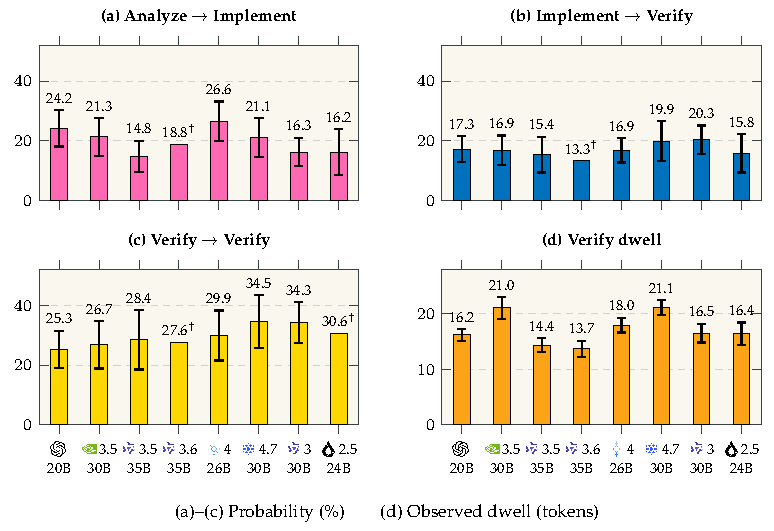
\includegraphics[width=\linewidth]{figures/journal/transition_summary.pdf}
\caption{Observed transitions from Analyze to Implement (a), Implement to Verify (b), and Verify to Verify (c), with Verify dwell (d).
%
Transition panels share a percentage scale.
%
Dwell counts labelled tokens in an observed run and can be censored by missing-label boundaries.
%
Horizontal values give means.
%
Whiskers show the whole-family-bootstrap, model-specific simultaneous 95\% intervals.
%
A dagger marks unavailable transition intervals.
%
These endpoints describe observed state dynamics.}
\label{fig:transition-summary}
\end{figure}

% Necessary local flush: the state/dwell figure must remain in Appendix C.
\FloatBarrier
\journalappendix{Benchmark Denominators and Model Configurations}{app:benchmark-details}

The complete native score table retains all six benchmark cells for every evaluated model (Table~\ref{tab:benchmark-details}).
%
The intervals are the original source-question bootstrap intervals.
%
The 32 attempts for each competition question remain dependent measurements, and unresolved answers are excluded from the scored denominator.
%

% Multipage longtable: retained outside adjustbox so page breaks remain available.
% Compact 2pt intercolumn spacing fits the full model identities without text scaling.
% Adapted from SPSD tab:main-results and SYNCO tab:mainRes.
\begingroup\small
\setlength{\tabcolsep}{2pt}
\begin{longtable}{llrrc}
\caption{\protect\phantomsection\label{tab:benchmark-details}Mean native card-profile accuracy (\%) with question-bootstrap 95\% confidence intervals in subscripts.
%
Repeated attempts remain grouped by source question.
%
Scored counts retain unresolved-answer exclusions.
%
Bold and underline mark the highest and second-highest unrounded means per benchmark, with ties sharing a rank, as in Table~\ref{tab:benchmarks}.}\\
\toprule
Model & Benchmark & Questions & Scored & Mean accuracy (\%) \\
\midrule\endfirsthead
\multicolumn{5}{l}{\textit{Continued}}\\
\toprule
Model & Benchmark & Questions & Scored & Mean accuracy (\%) \\
\midrule\endhead
\bottomrule\endfoot
\modelname{openai}{GPT-OSS-20B} & AIME24 & 30 & 956 & \cid{78.7}{13.0}{9.7} \\
\modelname{openai}{GPT-OSS-20B} & AIME25 & 30 & 956 & \cid{76.0}{11.4}{10.0} \\
\modelname{openai}{GPT-OSS-20B} & AMC23 & 40 & 1278 & \cid{97.3}{2.7}{2.1} \\
\modelname{openai}{GPT-OSS-20B} & MATH-500 & 500 & 500 & \cid{97.0}{1.6}{1.4} \\
\modelname{openai}{GPT-OSS-20B} & Minerva Math & 272 & 272 & \cid{69.1}{5.9}{5.5} \\
\modelname{openai}{GPT-OSS-20B} & OlympiadBench & 675 & 674 & \cid{83.2}{2.8}{2.7} \\
\modelname{nvidia}{\shortstack[l]{Nemotron-3.5-Lightning\\30B-A3B}} & AIME24 & 30 & 960 & \cid{87.8}{12.5}{8.8} \\
\modelname{nvidia}{\shortstack[l]{Nemotron-3.5-Lightning\\30B-A3B}} & AIME25 & 30 & 960 & \cid{87.2}{11.3}{9.2} \\
\modelname{nvidia}{\shortstack[l]{Nemotron-3.5-Lightning\\30B-A3B}} & AMC23 & 40 & 1280 & \secondcid{99.8}{0.3}{0.2} \\
\modelname{nvidia}{\shortstack[l]{Nemotron-3.5-Lightning\\30B-A3B}} & MATH-500 & 500 & 500 & \cid{98.8}{1.0}{0.8} \\
\modelname{nvidia}{\shortstack[l]{Nemotron-3.5-Lightning\\30B-A3B}} & Minerva Math & 272 & 272 & \cid{73.5}{5.9}{5.1} \\
\modelname{nvidia}{\shortstack[l]{Nemotron-3.5-Lightning\\30B-A3B}} & OlympiadBench & 675 & 675 & \cid{88.6}{2.4}{2.4} \\
\modelname{qwen}{Qwen3.5-35B-A3B} & AIME24 & 30 & 960 & \secondcid{94.0}{8.6}{5.4} \\
\modelname{qwen}{Qwen3.5-35B-A3B} & AIME25 & 30 & 960 & \cid{88.3}{11.3}{9.8} \\
\modelname{qwen}{Qwen3.5-35B-A3B} & AMC23 & 40 & 1280 & \bestcid{100.0}{0.0}{0.0} \\
\modelname{qwen}{Qwen3.5-35B-A3B} & MATH-500 & 500 & 500 & \secondcid{99.4}{0.8}{0.6} \\
\modelname{qwen}{Qwen3.5-35B-A3B} & Minerva Math & 272 & 271 & \cid{73.4}{5.5}{5.5} \\
\modelname{qwen}{Qwen3.5-35B-A3B} & OlympiadBench & 675 & 675 & \bestcid{92.3}{2.1}{2.1} \\
\modelname{qwen}{Qwen3.6-35B-A3B} & AIME24 & 30 & 960 & \bestcid{94.8}{7.1}{5.0} \\
\modelname{qwen}{Qwen3.6-35B-A3B} & AIME25 & 30 & 960 & \bestcid{89.7}{10.9}{9.2} \\
\modelname{qwen}{Qwen3.6-35B-A3B} & AMC23 & 40 & 1280 & \bestcid{100.0}{0.0}{0.0} \\
\modelname{qwen}{Qwen3.6-35B-A3B} & MATH-500 & 500 & 500 & \bestcid{99.6}{0.6}{0.4} \\
\modelname{qwen}{Qwen3.6-35B-A3B} & Minerva Math & 272 & 270 & \secondcid{74.8}{5.6}{5.2} \\
\modelname{qwen}{Qwen3.6-35B-A3B} & OlympiadBench & 675 & 675 & \secondcid{92.0}{2.1}{1.9} \\
\modelname{gemma}{Gemma-4-26B-A4B} & AIME24 & 30 & 959 & \cid{90.8}{9.8}{7.2} \\
\modelname{gemma}{Gemma-4-26B-A4B} & AIME25 & 30 & 948 & \cid{86.8}{10.5}{8.8} \\
\modelname{gemma}{Gemma-4-26B-A4B} & AMC23 & 40 & 1280 & \cid{99.7}{0.6}{0.3} \\
\modelname{gemma}{Gemma-4-26B-A4B} & MATH-500 & 500 & 500 & \cid{99.0}{1.0}{0.8} \\
\modelname{gemma}{Gemma-4-26B-A4B} & Minerva Math & 272 & 271 & \bestcid{75.6}{4.8}{5.2} \\
\modelname{gemma}{Gemma-4-26B-A4B} & OlympiadBench & 675 & 674 & \cid{90.8}{2.2}{2.1} \\
\modelname{zhipu}{GLM-4.7-Flash (30B-A3B)} & AIME24 & 30 & 960 & \cid{93.2}{7.7}{4.9} \\
\modelname{zhipu}{GLM-4.7-Flash (30B-A3B)} & AIME25 & 30 & 960 & \secondcid{89.6}{9.7}{7.6} \\
\modelname{zhipu}{GLM-4.7-Flash (30B-A3B)} & AMC23 & 40 & 1280 & \cid{99.4}{0.5}{0.4} \\
\modelname{zhipu}{GLM-4.7-Flash (30B-A3B)} & MATH-500 & 500 & 500 & \cid{98.4}{1.2}{1.0} \\
\modelname{zhipu}{GLM-4.7-Flash (30B-A3B)} & Minerva Math & 272 & 271 & \cid{73.1}{5.5}{5.2} \\
\modelname{zhipu}{GLM-4.7-Flash (30B-A3B)} & OlympiadBench & 675 & 674 & \cid{90.5}{2.2}{2.1} \\
\modelname{qwen}{Qwen3-30B-A3B} & AIME24 & 30 & 960 & \cid{80.2}{14.7}{11.0} \\
\modelname{qwen}{Qwen3-30B-A3B} & AIME25 & 30 & 960 & \cid{71.1}{13.3}{12.1} \\
\modelname{qwen}{Qwen3-30B-A3B} & AMC23 & 40 & 1280 & \cid{97.7}{2.5}{1.8} \\
\modelname{qwen}{Qwen3-30B-A3B} & MATH-500 & 500 & 500 & \cid{98.0}{1.2}{1.2} \\
\modelname{qwen}{Qwen3-30B-A3B} & Minerva Math & 272 & 271 & \bestcid{75.6}{5.2}{4.8} \\
\modelname{qwen}{Qwen3-30B-A3B} & OlympiadBench & 675 & 674 & \cid{84.6}{2.8}{2.5} \\
\modelname{liquid}{LFM2.5-24B-A2B} & AIME24 & 30 & 960 & \cid{86.9}{12.3}{8.4} \\
\modelname{liquid}{LFM2.5-24B-A2B} & AIME25 & 30 & 960 & \cid{84.4}{9.9}{8.6} \\
\modelname{liquid}{LFM2.5-24B-A2B} & AMC23 & 40 & 1280 & \cid{97.9}{2.3}{1.7} \\
\modelname{liquid}{LFM2.5-24B-A2B} & MATH-500 & 500 & 500 & \cid{98.8}{1.0}{0.8} \\
\modelname{liquid}{LFM2.5-24B-A2B} & Minerva Math & 272 & 271 & \cid{74.2}{5.7}{5.2} \\
\modelname{liquid}{LFM2.5-24B-A2B} & OlympiadBench & 675 & 675 & \cid{89.0}{2.5}{2.2} \\
\end{longtable}
\endgroup


\subsection{Model identities}
The evaluated models are OpenAI's GPT-OSS-20B, NVIDIA's Nemotron-3.5-Lightning-30B-A3B-NVFP4, Qwen3.5-35B-A3B-GPTQ-Int4, Qwen3.6-35B-A3B-FP8, NVIDIA's Gemma-4-26B-A4B-NVFP4, Z.ai's GLM-4.7-Flash, Qwen3-30B-A3B, and LiquidAI's LFM2.5-24B-A2B.
%
The native evaluation retains their model-specific tokenizers and reasoning parsers.
%
GPT-OSS has a 131,072-token context capacity.
%
The retained five long-context profiles use 133,120 tokens, while Qwen3-30B uses 40,960.
%
Its output cap is 38,912 tokens.
%
The five long-context card profiles have a 131,072-token output cap, and GPT-OSS output is bounded by the remaining context.
%
LFM2.5 runs in BF16 with a 131,072-token context, and its output is bounded by the remaining context.
%
Its 38 routed layers follow two dense layers and use sigmoid selection scores with a correction bias.
%

\subsection{Native benchmark prompt}
\label{app:native-prompt}

The eight evaluated models receive the same user-message template for these benchmarks.
%
The problem text replaces the italicized field.
%
\begin{quote}\small
Please reason step by step, and put your final answer within \verb|\boxed{}|.\\ Question: \emph{problem text}
\end{quote}
There are no few-shot examples or separate system messages.
%
Each model uses its native chat template.
%
Gemma and LFM2.5 explicitly enable thinking, and GPT-OSS uses medium reasoning effort.
%
The other profiles retain their native thinking settings without a template override.
%
These conditions describe the completed native evaluation.
%

\journalappendix{Annotation and External Prefix Probes}{app:annotation}

\subsection{Native sentence sampling and token alignment}

Native reasoning regions are identified using each model's reasoning delimiters.
%
A deterministic punctuation/newline splitter protects mathematical expressions and records exact character offsets.
%
It splits the reasoning region into sentence units, rather than applying a learned linguistic parser.
%
A completion token belongs to the sentence with greatest character overlap.
%
Ties choose the earlier sentence, and whitespace gaps attach to the preceding sentence.
%
Delimiter and answer tokens have no sentence owner.
%

One uniformly sampled attempt per question defines the native allocation population.
%
Within those attempts, the annotation floor samples up to ten sentences without replacement.
%
Remaining assignments sample the pooled unused sentences toward the 100,000-unit budget.
%
A separate competition sample includes up to four successful and four unsuccessful attempts from questions having at least two of each.
%
It assigns up to 60 sentences per attempt.
%
When an attempt overlaps the allocation population, its sentence assignments are unioned, so the available union can exceed the nominal budget.
%
Unscored attempts are not assigned to its success/failure strata.
%
The allocation comparison continues to use its original single sampled attempt per question.
%
Unassigned, invalid or unavailable labels remain missing and break sentence adjacency.
%

\subsection{External annotation development}

The external annotation development corpus contains 38 released DeepSeek-R1 SAT responses and 3,125 labelled units.
%
Complete responses define the partitions before units are flattened.
%
The Qwen3.8 seed deployment check uses 407 reused validation units, obtaining accuracy 0.710 under both low and medium effort.
%
The settings change 41 labels, or 10.1\% of those units.
%
Equal aggregate accuracy therefore does not imply an unchanged set of individual judgments.
%

The retained prompt has balanced accuracy 0.7400 in its selection comparison, against 0.7288 for the optimized candidate.
%
The Plan-recall gate retains the seed.
%
An earlier response-grouped, static-reward prompt study obtains macro-F1 0.6505 with a light optimization budget and 0.6437 with a heavy budget over 2,789 units.
%
These are different development comparisons, and their scores do not supply native seven-model annotation accuracy.
%

\subsection{Lexical reading of intervention continuations}
\label{app:lexical-readout}

The state of an intervention continuation is assigned by a text classifier rather than by the annotation reader.
%
It receives the sentence and its two neighbours, the same text the reader sees apart from the problem statement.
%
Word unigrams and bigrams and character 3- to 5-grams of the sentence, and word unigrams and bigrams of each neighbour, enter as hashed sublinear TF-IDF blocks fitted on the training rows.
%
The neighbour blocks carry half the weight of the sentence block, and nine format features record length, digit and symbol density, closing question marks or colons, bullets, and the response-boundary markers.
%
A multinomial logistic regression with an $L_2$ penalty maps these features to the seven classes.
%

Training uses the reader-labelled native sentences of the seven source models, at most 60,000 unique contexts per model and 420,000 in total.
%
Each evaluation fold has its own classifier, fitted on the families of the other four folds, so no continuation is read by a classifier that saw its question family.
%
On held-out native sentences the classifier agrees with the reader on 73.4\% of labels, with macro-F1 0.696 and per-model accuracy between 72.0\% and 75.0\%.
%
Its Youden index, sensitivity minus false-positive rate, ranges from 0.42 for Read to 0.74 for Implement.
%
The reader itself agrees with a repeated judgment of the same context in 83 to 95\% of duplicated contexts, which bounds the agreement any reader-trained classifier can reach.
%
LFM2.5 contributes no training sentence.
%
On its 96,137 reader-labelled native contexts, the same fold-specific classifiers agree with the reader on 72.7\% of labels, with macro-F1 0.672 and Youden indices between 0.37 for Read and 0.74 for Implement.
%

Non-differential classification errors shrink a contrast in class occupancy by the Youden index of that class without changing its sign.
%
The main analysis therefore reports uncorrected occupancy contrasts and gives Rogan--Gladen corrections, which divide by the native Youden index, as a sensitivity analysis.
%
On 27,746 reader-labelled sentences from an earlier steering study, an equivalent classifier reaches 74.4\% agreement, and its accuracy differs between targeted and random arms by 0.3 points with a 95\% interval from $-0.8$ to $1.4$.
%
Classifier contrasts between those arms correlate with reader contrasts at $r=0.71$, with a slope consistent with the Youden attenuation.
%
These checks cover a single model and milder edits, so the readout supports statements about lexical signatures of the reasoning classes rather than independently verified cognitive states.
%

\subsection{Prospective hidden-state information}
\label{app:probes}

The external prefix-probe study removes 38 synthetic closing-think units, leaving 3,087 annotated units.
%
The feature for a sentence is the hidden state immediately before its first token.
%
Each encoder receives the released response as a teacher-forced continuation.
%
The probe therefore observes the problem and preceding text without the target sentence.
%

The probes use balanced one-versus-rest logistic regression with L2 regularization, $C=1$, and raw hidden activations without standardization or principal-component reduction.
%
Five common response-disjoint outer folds hold out complete responses.
%
Inner validation selects the layer for each one-versus-rest target by area under the receiver operating characteristic curve (AUROC), and the selected classifier is refitted on the outer development responses.
%
A position-only baseline uses the logarithms of preceding unit and token counts, without future content or final response length.
%

\begin{table}[htbp]
\centering\small
\caption{Response-disjoint prospective probes on 38 SAT responses.
%
AUROC averages the five folds and seven binary targets.
%
Subscripts give $\pm$ 95\% response-bootstrap confidence intervals, conditional on the saved folds, layers, and fits.
%
Gain subtracts the position baseline.
%
Bold and underline identify the highest and second-highest distinct probe AUROC and paired gain.
%
Probes use encoder-specific representations.}
\label{tab:prefix-probes}
\begin{adjustbox}{max width=\linewidth}
\begin{tabular}{@{}lrrr@{}}
\toprule
Encoder & Probe AUROC & Position AUROC & Paired gain \\
\midrule
\modelname{qwen}{Qwen3.5-35B-A3B} & \bestcid{0.852}{0.014}{0.016} & \cid{0.566}{0.014}{0.028} & \bestcid{0.286}{0.027}{0.016} \\
\modelname{openai}{GPT-OSS-20B} & \cid{0.780}{0.019}{0.017} & \cid{0.571}{0.014}{0.029} & \cid{0.209}{0.030}{0.018} \\
\modelname{gemma}{Gemma-4-26B-A4B} & \secondcid{0.788}{0.016}{0.017} & \cid{0.566}{0.013}{0.028} & \secondcid{0.221}{0.026}{0.016} \\
\bottomrule
\end{tabular}
\end{adjustbox}
\end{table}

Every encoder exceeds its position baseline (Table~\ref{tab:prefix-probes}).
%
The intervals resample whole responses and condition on the chosen layers and fitted classifiers.
%
They omit refitting and split-seed variation.
%
Macro binary F1 is 0.521 for Qwen3.5, 0.400 for GPT-OSS, and 0.426 for Gemma at the retained decision rule.
%
Ranking information does not therefore establish reliable seven-class annotation of a model's own generated solutions.
%

\subsection{Candidate-specific verification qualification}
\label{app:verification-qualification}

The separate prospective verification protocol recognizes a checkable candidate value inside an already emitted reasoning prefix.
%
Its frozen qualification combines family support, precision, and evidence of whether that candidate has already been checked.
%
The completed recognition audits do not qualify in five models.
%
Qwen3.5 and GLM remain incomplete under that protocol (Table~\ref{tab:verification-qualification}).
%
No new targeted-control outcome is measured for these seven protocol cells.
%

\begin{table}[htb]
\centering\small
\caption{Qualification of the separate candidate-specific verification protocol.
%
Engineering qualification concerns execution.
%
Recognition and targeted-control outcomes are assessed separately.}
\label{tab:verification-qualification}
\begin{adjustbox}{max width=\linewidth}
\begin{tabular}{@{}llll@{}}
\toprule
Model & Engineering & Recognition & Targeted control \\
\midrule
\modelname{openai}{GPT-OSS-20B} & Qualified & Criterion unmet & Unmeasured \\
\modelname{nvidia}{\shortstack[l]{Nemotron-3.5-Lightning\\30B-A3B}} & Qualified & Criterion unmet & Unmeasured \\
\modelname{qwen}{Qwen3.5-35B-A3B} & Qualified & Incomplete & Unmeasured \\
\modelname{qwen}{Qwen3.6-35B-A3B} & Qualified & Criterion unmet & Unmeasured \\
\modelname{gemma}{Gemma-4-26B-A4B} & Qualified & Criterion unmet & Unmeasured \\
\modelname{zhipu}{GLM-4.7-Flash (30B-A3B)} & Qualified & Incomplete & Unmeasured \\
\modelname{qwen}{Qwen3-30B-A3B} & Qualified & Criterion unmet & Unmeasured \\
\bottomrule
\end{tabular}
\end{adjustbox}
\end{table}

GPT-OSS's complete audit has 128 prefix assignments and two original reader draws per assignment.
%
Apparent eligibility precision is 22.41\% across 29 families, and already-checked precision is 18.75\% across eight families.
%
The frozen thresholds are 70\% precision and ten families for each qualification.
%
Both measured precisions fall below that criterion, and already-checked support also falls below ten families.
%
These results limit this recognition procedure's applicability.
%
An unmeasured control outcome does not estimate a causal null.

% Necessary local flush: the qualification float belongs to Appendix E.
\FloatBarrier
\journalappendix{Exploratory Correctness Associations}{app:associations}

An exploratory analysis relates whole-reasoning use of class-enriched expert sets to adjudicated correctness.
%
The retained rule nominates up to three experts per selected layer for each class on the full allocation corpus, without using correctness to rank them.
%
Their selected-slot use is measured over all reasoning tokens, including tokens outside the class used for nomination.
%
The class sets can overlap.
%

The original partial Pearson correlations adjust for benchmark, log completion length, retrospective difficulty, the labelled class's token share, and a cap indicator when present.
%
Difficulty uses other attempts on repeated competition questions or the other models on single-attempt benchmarks.
%
It is a retrospective adjustment variable.
%

The strongest corrected associations occur in Qwen3.5 and Qwen3.6.
%
Analyze-profile use has $r=0.0918$ and $r=0.0818$, while Verify-profile use has $r=-0.0972$ and $r=-0.1008$.
%
The Monitor-profile correlations are $-0.0770$ and $-0.0995$.
%
Nemotron's Monitor association is $-0.0853$.
%
The remaining tested mean-feature associations do not pass the original corrected threshold.
%

That threshold applies Benjamini--Hochberg correction within each model's 21 mean-feature comparisons~\citep{benjamini1995fdr}.
%
The original intervals use 1,000 question-ID bootstrap draws, refitting nuisance regressions while holding nominated sets and difficulty fixed.
%
They do not cluster duplicate families.
%
This is same-cohort association evidence.
%
It does not supply held-out expert usefulness or the effect of removing a class-associated expert.
%

\journalappendix{Paired Routing Interventions}{app:routing-levels}

Table~\ref{tab:routing-levels} gives the accuracy and token levels behind the paired contrasts of Section~\ref{sec:routing-results}.
%
Native routing ends naturally in at least 98\% of continuations in every model, and no edited arm changes this share by more than one point.
%
The levels carry wider intervals than the paired contrasts because they retain the variation between families that pairing removes.
%

% Multipage longtable: retained outside adjustbox so page breaks remain available.
% Source: analysis-final/EFFECTS.json levels_by_model via scripts/paper/export_routing_results.py.
\begingroup\small
\setlength{\tabcolsep}{2pt}
\begin{longtable}{lcccc}
\caption{Accuracy and token levels of every intervention arm, with family-bootstrap simultaneous 95\% confidence intervals as subscripts.
%
Accuracy is strict answer scoring of the completed continuation.
%
Generated tokens follow the frozen prefix, and reasoning tokens are the generated tokens before the reasoning closes.
%
Random arms use the matched control sets, and natural end is the share of continuations that stop before their original generation allowance.
%
Benchmarks and supported families receive equal weight, and intervals are simultaneous over the arm and metric cells of each model.}\label{tab:routing-levels}\\
\toprule
Arm & Accuracy (\%) & Generated tokens & Reasoning tokens & Natural end (\%) \\
\midrule\endfirsthead
\multicolumn{5}{l}{\textit{Continued}}\\
\toprule
Arm & Accuracy (\%) & Generated tokens & Reasoning tokens & Natural end (\%) \\
\midrule\endhead
\bottomrule\endfoot
\multicolumn{5}{l}{\modelname{openai}{GPT-OSS-20B}}\\*
Native & \cid{78.06}{9.18}{9.18} & \cid{3838}{1429}{1429} & \cid{3340}{1409}{1409} & \cid{100.0}{0.0}{0.0} \\*
Targeted activation & \cid{77.18}{8.17}{8.17} & \cid{3735}{1142}{1142} & \cid{3258}{1128}{1128} & \cid{100.0}{0.0}{0.0} \\*
Random activation & \cid{77.74}{8.13}{8.13} & \cid{3758}{1127}{1127} & \cid{3284}{1112}{1112} & \cid{100.0}{0.0}{0.0} \\*
Targeted deactivation & \cid{75.95}{8.34}{8.34} & \cid{3726}{1188}{1188} & \cid{3258}{1175}{1175} & \cid{100.0}{0.0}{0.0} \\*
Random deactivation & \cid{75.95}{8.22}{8.22} & \cid{3672}{1225}{1225} & \cid{3217}{1202}{1202} & \cid{100.0}{0.0}{0.0} \\
\midrule
\multicolumn{5}{l}{\modelname{nvidia}{Nemotron-3.5-Lightning-30B-A3B}}\\*
Native & \cid{84.73}{7.37}{7.37} & \cid{8034}{2846}{2846} & \cid{7675}{2853}{2853} & \cid{100.0}{0.0}{0.0} \\*
Targeted activation & \cid{84.53}{6.82}{6.82} & \cid{7363}{2390}{2390} & \cid{6986}{2395}{2395} & \cid{100.0}{0.0}{0.0} \\*
Random activation & \cid{83.46}{7.09}{7.09} & \cid{7632}{2597}{2597} & \cid{7257}{2602}{2602} & \cid{100.0}{0.0}{0.0} \\*
Targeted deactivation & \cid{83.94}{7.12}{7.12} & \cid{7763}{2613}{2613} & \cid{7392}{2619}{2619} & \cid{100.0}{0.0}{0.0} \\*
Random deactivation & \cid{83.62}{7.00}{7.00} & \cid{7416}{2464}{2464} & \cid{7044}{2468}{2468} & \cid{100.0}{0.0}{0.0} \\
\midrule
\multicolumn{5}{l}{\modelname{qwen}{Qwen3.5-35B-A3B}}\\*
Native & \cid{87.78}{7.12}{7.12} & \cid{9838}{2580}{2580} & \cid{8890}{2610}{2610} & \cid{100.0}{0.0}{0.0} \\*
Targeted activation & \cid{87.22}{6.76}{6.76} & \cid{10442}{2945}{2945} & \cid{9470}{2960}{2960} & \cid{100.0}{0.0}{0.0} \\*
Random activation & \cid{87.46}{7.04}{7.04} & \cid{10288}{2746}{2746} & \cid{9326}{2747}{2747} & \cid{99.9}{0.2}{0.2} \\*
Targeted deactivation & \cid{87.02}{7.03}{7.03} & \cid{10252}{2787}{2787} & \cid{9270}{2792}{2792} & \cid{100.0}{0.0}{0.0} \\*
Random deactivation & \cid{87.54}{7.02}{7.02} & \cid{9954}{2769}{2769} & \cid{8991}{2779}{2779} & \cid{100.0}{0.0}{0.0} \\
\midrule
\multicolumn{5}{l}{\modelname{qwen}{Qwen3.6-35B-A3B}}\\*
Native & \cid{87.50}{6.29}{6.29} & \cid{11828}{3464}{3464} & \cid{11149}{3461}{3461} & \cid{100.0}{0.0}{0.0} \\*
Targeted activation & \cid{85.79}{7.01}{7.01} & \cid{11273}{3395}{3395} & \cid{10597}{3390}{3390} & \cid{99.8}{0.4}{0.4} \\*
Random activation & \cid{86.39}{6.84}{6.84} & \cid{11806}{4065}{4065} & \cid{11133}{4066}{4066} & \cid{99.5}{1.2}{1.2} \\*
Targeted deactivation & \cid{86.27}{6.42}{6.42} & \cid{11633}{3978}{3978} & \cid{10961}{3980}{3980} & \cid{99.2}{2.0}{2.0} \\*
Random deactivation & \cid{85.87}{6.56}{6.56} & \cid{11532}{4007}{4007} & \cid{10856}{4005}{4005} & \cid{99.4}{1.6}{1.6} \\
\midrule
\multicolumn{5}{l}{\modelname{gemma}{Gemma-4-26B-A4B}}\\*
Native & \cid{85.83}{7.57}{7.57} & \cid{8278}{4156}{4156} & \cid{7519}{4186}{4186} & \cid{98.1}{3.9}{3.9} \\*
Targeted activation & \cid{84.88}{7.53}{7.53} & \cid{7735}{2733}{2733} & \cid{6959}{2743}{2743} & \cid{98.5}{2.3}{2.3} \\*
Random activation & \cid{83.85}{7.57}{7.57} & \cid{8091}{3335}{3335} & \cid{7016}{3258}{3258} & \cid{98.0}{2.7}{2.7} \\*
Targeted deactivation & \cid{84.05}{7.43}{7.43} & \cid{8141}{2999}{2999} & \cid{7389}{3019}{3019} & \cid{98.1}{2.3}{2.3} \\*
Random deactivation & \cid{84.44}{7.54}{7.54} & \cid{7679}{2556}{2556} & \cid{6920}{2572}{2572} & \cid{98.4}{2.1}{2.1} \\
\midrule
\multicolumn{5}{l}{\modelname{zhipu}{GLM-4.7-Flash (30B-A3B)}}\\*
Native & \cid{85.00}{7.48}{7.48} & \cid{9093}{3432}{3432} & \cid{8638}{3437}{3437} & \cid{98.3}{2.5}{2.5} \\*
Targeted activation & \cid{84.64}{7.13}{7.13} & \cid{9139}{3687}{3687} & \cid{8705}{3683}{3683} & \cid{98.5}{2.3}{2.3} \\*
Random activation & \cid{84.76}{6.66}{6.66} & \cid{9094}{3792}{3792} & \cid{8670}{3793}{3793} & \cid{98.4}{2.4}{2.4} \\*
Targeted deactivation & \cid{84.64}{7.32}{7.32} & \cid{9425}{3785}{3785} & \cid{9000}{3783}{3783} & \cid{98.3}{2.3}{2.3} \\*
Random deactivation & \cid{84.76}{7.02}{7.02} & \cid{9368}{3602}{3602} & \cid{8948}{3602}{3602} & \cid{98.3}{2.3}{2.3} \\
\midrule
\multicolumn{5}{l}{\modelname{qwen}{Qwen3-30B-A3B}}\\*
Native & \cid{79.73}{9.81}{9.81} & \cid{6130}{1403}{1403} & \cid{5305}{1392}{1392} & \cid{99.4}{1.5}{1.5} \\*
Targeted activation & \cid{78.57}{9.02}{9.02} & \cid{6554}{1430}{1430} & \cid{5741}{1418}{1418} & \cid{99.0}{1.9}{1.9} \\*
Random activation & \cid{77.95}{9.60}{9.60} & \cid{6411}{1433}{1433} & \cid{5607}{1430}{1430} & \cid{99.4}{1.5}{1.5} \\*
Targeted deactivation & \cid{77.67}{9.76}{9.76} & \cid{6399}{1376}{1376} & \cid{5582}{1369}{1369} & \cid{98.9}{1.8}{1.8} \\*
Random deactivation & \cid{78.26}{9.04}{9.04} & \cid{6308}{1322}{1322} & \cid{5488}{1304}{1304} & \cid{99.4}{1.5}{1.5} \\
\midrule
\multicolumn{5}{l}{\modelname{liquid}{LFM2.5-24B-A2B}}\\*
Native & \cid{85.43}{8.23}{8.23} & \cid{9706}{5597}{5597} & \cid{9384}{5608}{5608} & \cid{99.4}{1.7}{1.7} \\*
Targeted activation & \cid{84.37}{7.73}{7.73} & \cid{8637}{5018}{5018} & \cid{8319}{5033}{5033} & \cid{99.0}{1.8}{1.8} \\*
Random activation & \cid{83.93}{7.81}{7.81} & \cid{9620}{4846}{4846} & \cid{9304}{4856}{4856} & \cid{99.0}{1.9}{1.9} \\*
Targeted deactivation & \cid{84.01}{7.56}{7.56} & \cid{8856}{4310}{4310} & \cid{8534}{4322}{4322} & \cid{98.8}{1.9}{1.9} \\*
Random deactivation & \cid{84.76}{7.44}{7.44} & \cid{8464}{4378}{4378} & \cid{8138}{4390}{4390} & \cid{99.1}{1.8}{1.8} \\
\end{longtable}
\endgroup


\subsection{Pre-registered efficiency link}
\label{app:efficiency-link}

The efficiency link was frozen on native traces before any intervention outcome existed.
%
For each model and class, a regression of the log remaining reasoning tokens on the class indicator absorbs question and absolute-position fixed effects, without relative position or trace effects that would leak the outcome (Table~\ref{tab:efficiency-link}).
%
Its intervals use 2,000 family-bootstrap resamples with seed 20261017, shared across models, classes and outcomes.
%
The prediction states that the token effect of targeted activation relative to matched random activation correlates positively with this coefficient across model--class cells, and that the accuracy effect correlates positively with the corresponding correctness coefficient.
%
The test reports the Spearman correlation and the sign-agreement rate over cells whose native interval excludes zero.
%
LFM2.5 has no frozen coefficient because its labels became available after the pre-registration.
%

% Source: report/final-routing-20261015-r1/driver/EFFICIENCY_LINK_PREREG.json via scripts/paper/export_routing_results.py.
\begin{table}[tb]
\centering\small
\caption{Pre-registered native association between the current reasoning state and the remaining reasoning length, with 95\% family-bootstrap confidence intervals as subscripts.
%
Entries are 100 times the regression coefficient of a class indicator on the log of the reasoning tokens that remain after the sentence, with question and absolute-position fixed effects.
%
Negative values mark states followed by shorter remaining reasoning.
%
The coefficients were frozen before any intervention outcome existed.}
\label{tab:efficiency-link}
\setlength{\tabcolsep}{2pt}
\begin{adjustbox}{max width=\linewidth}
\begin{tabular}{@{}lccccccc@{}}
\toprule
Model & \textrm{Re} & \textrm{An} & \textrm{Ex} & \textrm{Pl} & \textrm{Im} & \textrm{Ve} & \textrm{Mo} \\
\midrule
\modelname{openai}{GPT-OSS-20B} & \cid{19.88}{2.60}{2.82} & \cid{11.58}{1.65}{1.82} & \cid{4.56}{1.67}{1.76} & \cid{8.98}{2.01}{2.00} & \cid{0.71}{1.81}{1.81} & \cid{-4.69}{1.93}{1.91} & \cid{-36.71}{3.74}{3.53} \\
\modelname{nvidia}{Nemotron-3.5-Lightning-30B-A3B} & \cid{10.43}{2.82}{2.93} & \cid{6.61}{1.21}{1.21} & \cid{0.22}{1.38}{1.45} & \cid{8.05}{1.65}{1.72} & \cid{2.81}{1.71}{1.70} & \cid{-4.79}{1.82}{1.73} & \cid{-30.76}{4.00}{3.83} \\
\modelname{qwen}{Qwen3.5-35B-A3B} & \cid{1.78}{2.22}{2.15} & \cid{4.09}{1.18}{1.15} & \cid{1.86}{1.60}{1.53} & \cid{4.01}{2.05}{2.11} & \cid{1.02}{1.47}{1.43} & \cid{-5.01}{1.66}{1.71} & \cid{-8.95}{1.95}{2.04} \\
\modelname{qwen}{Qwen3.6-35B-A3B} & \cid{-0.93}{2.47}{2.40} & \cid{5.57}{1.12}{1.25} & \cid{0.78}{1.39}{1.42} & \cid{4.06}{2.09}{1.99} & \cid{2.21}{1.45}{1.47} & \cid{-5.24}{1.90}{1.84} & \cid{-11.12}{1.81}{1.83} \\
\modelname{gemma}{Gemma-4-26B-A4B} & \cid{4.57}{2.06}{2.08} & \cid{5.91}{1.34}{1.36} & \cid{3.38}{2.06}{2.20} & \cid{4.07}{2.45}{2.58} & \cid{-2.35}{1.48}{1.42} & \cid{-7.57}{1.83}{1.75} & \cid{-3.40}{2.80}{2.77} \\
\modelname{zhipu}{GLM-4.7-Flash (30B-A3B)} & \cid{19.12}{3.81}{3.80} & \cid{7.43}{1.56}{1.69} & \cid{1.78}{1.97}{1.89} & \cid{2.02}{2.29}{2.38} & \cid{2.97}{1.96}{1.92} & \cid{-3.66}{1.78}{1.70} & \cid{-28.28}{3.77}{3.42} \\
\modelname{qwen}{Qwen3-30B-A3B} & \cid{4.60}{1.75}{1.81} & \cid{8.20}{1.24}{1.32} & \cid{4.51}{1.52}{1.41} & \cid{7.39}{1.40}{1.44} & \cid{2.46}{1.36}{1.36} & \cid{-6.88}{1.49}{1.46} & \cid{-18.32}{2.31}{2.22} \\
\midrule
Seven-model mean & \cid{8.49}{1.23}{1.31} & \cid{7.06}{0.57}{0.59} & \cid{2.44}{0.65}{0.65} & \cid{5.51}{0.82}{0.84} & \cid{1.40}{0.70}{0.67} & \cid{-5.41}{0.72}{0.71} & \cid{-19.65}{1.53}{1.36} \\
\bottomrule
\end{tabular}
\end{adjustbox}
\end{table}


Verify and Monitor precede shorter remaining reasoning in every model, and Analyze precedes longer remaining reasoning in every model.
%
The correctness coefficients are small, and only 20\% of the 49 cells exclude zero.
%
Neither prediction holds: the token correlation is $-0.11$, with a 95\% interval from $-0.29$ to $0.13$, and the accuracy correlation is $0.07$, from $-0.16$ to $0.31$.
%
Fixed effects for benchmark, total tokens instead of reasoning tokens, and accuracy restricted to completed traces give the same conclusion.
%

\subsection{Exploratory strong-dose arm}
\label{app:routing-strong}

The strong-dose arm was specified after the primary contrasts of three models had been inspected.
%
It reuses each family's native prefix and seed, and forces the high-count nominated sets of all three depth regions throughout the analysis window rather than for a pulse.
%
Its matched control forces the corresponding high-count control sets of the same layers.
%
The arm adds 7,196 continuations in GPT-OSS, Nemotron, Qwen3-30B and Gemma (Table~\ref{tab:routing-strong}).
%

% Source: report/final-routing-20261015-r1/driver/analysis-strong/EFFECTS.json via scripts/paper/export_routing_results.py.
\begin{table}[tb]
\centering\small
\caption{Exploratory strong-dose activation, with family-bootstrap simultaneous 95\% confidence intervals as subscripts.
%
The arm forces the nominated high-count expert sets at all three depth regions throughout the analysis window and compares them with the matched high-count control sets.
%
State columns give targeted minus matched-random percentage points.
%
Accuracy is in percentage points and generated tokens in percent; efficiency contrasts are estimated on the pooled population only.}
\label{tab:routing-strong}
\setlength{\tabcolsep}{2.5pt}
\begin{adjustbox}{max width=\linewidth}
\begin{tabular}{@{}lcccccc@{}}
\toprule
 & \multicolumn{2}{c}{Target state (pp)} & \multicolumn{2}{c}{Targeted $-$ random} & \multicolumn{2}{c}{Accuracy $-$ native (pp)} \\
\cmidrule(lr){2-3}\cmidrule(lr){4-5}\cmidrule(lr){6-7}
Model & Occupancy & First & Acc.\ (pp) & Tokens (\%) & Targeted & Random \\
\midrule
\modelname{openai}{GPT-OSS-20B} & \cid{-0.19}{0.93}{0.93} & \cid{0.08}{1.58}{1.58} & \textemdash & \textemdash & \textemdash & \textemdash \\
\modelname{nvidia}{Nemotron-3.5-Lightning-30B-A3B} & \cid{0.02}{0.95}{0.95} & \cid{0.42}{1.67}{1.67} & \textemdash & \textemdash & \textemdash & \textemdash \\
\modelname{qwen}{Qwen3-30B-A3B} & \cid{0.09}{0.98}{0.98} & \cid{-0.02}{1.15}{1.15} & \textemdash & \textemdash & \textemdash & \textemdash \\
\modelname{gemma}{Gemma-4-26B-A4B} & \cid{0.23}{0.85}{0.85} & \cid{0.48}{0.88}{0.88} & \textemdash & \textemdash & \textemdash & \textemdash \\
\midrule
All four models & \cid{0.04}{0.46}{0.46} & \cid{0.27}{0.76}{0.76} & \cid{-0.17}{1.22}{1.22} & \cid{0.2}{3.1}{3.1} & \cid{-1.52}{2.18}{2.18} & \cid{-1.35}{2.37}{2.37} \\
\bottomrule
\end{tabular}
\end{adjustbox}
\end{table}


Neither occupancy nor the first sentence moves toward the forced class beyond the matched control.
%
Both forced arms lower mean accuracy relative to native routing, with simultaneous intervals that include zero.
%
Sustained routing edits therefore leave the state unchanged even when they persist across the whole window.
%

\journalappendix{Whole-Reasoning Steering}{app:whole}

This appendix details the whole-reasoning steering of Section~\ref{sec:whole-steering}.
%
Table~\ref{tab:whole-cells} gives the token and accuracy effect of every steered cell at each model's base strength, against matched random edits and against native routing.
%
Table~\ref{tab:whole-occupancy} gives the response $\rho$ of the steered state's occupancy, signed so that positive values move the state in the intended direction.
%
Table~\ref{tab:whole-levels} gives, for every model, strength and arm, the completed continuations, the share that reaches the length limit, the share of repeated 16-token windows, the mean generated tokens and the share of router positions at which the edit changed the selected experts.
%

Three design choices were fixed before any production outcome.
%
The pre-production check stopped a model only for breakdown, after its length-ratio criterion was removed, and GPT-OSS-20B and GLM-4.7-Flash ran their base continuations at half strength (Section~\ref{sec:whole-setup}).
%
The random experts are drawn separately at each strength, so the strength comparison varies the matched control together with the targeted set.
%

% Multipage longtable: retained outside adjustbox so page breaks remain available.
% Source: report/whole-reasoning-20261021-r14/analysis-combined/EFFECTS_WHOLE.json (cell_effects, levels) via scripts/paper/export_whole_results.py.
\begingroup\small
\setlength{\tabcolsep}{2pt}
\begin{longtable}{lccccc}
\caption{Effects of every steered cell at each model's base strength, with family-bootstrap simultaneous 95\% confidence intervals as subscripts.
%
Re, An, Ex, Pl, Im, Ve and Mo abbreviate Read, Analyze, Explore, Plan, Implement, Verify and Monitor.
%
A dagger marks the efficiency-directed cells that enter the primary contrast.
%
Tokens give the percent change in reasoning tokens, with negative values meaning fewer tokens, and accuracy differences are in percentage points, for targeted edits against matched random edits and against native routing.
%
Limit gives the share of the targeted continuations of each operation that reach the length limit.
%
Intervals are simultaneous over the six contrasts of each cell and cover the outcome bounds of unfinished continuations.
%
Each model is shown at its base strength, which is full except for GPT-OSS-20B and GLM-4.7-Flash at half.}\label{tab:whole-cells}\\
\toprule
 & \multicolumn{2}{c}{Targeted $-$ random} & \multicolumn{2}{c}{Targeted $-$ native} & \\
\cmidrule(lr){2-3}\cmidrule(lr){4-5}
Cell & Tokens (\%) & Acc.\ (pp) & Tokens (\%) & Acc.\ (pp) & Limit (\%) \\
\midrule\endfirsthead
\multicolumn{6}{l}{\textit{Continued}}\\
\toprule
 & \multicolumn{2}{c}{Targeted $-$ random} & \multicolumn{2}{c}{Targeted $-$ native} & \\
\cmidrule(lr){2-3}\cmidrule(lr){4-5}
Cell & Tokens (\%) & Acc.\ (pp) & Tokens (\%) & Acc.\ (pp) & Limit (\%) \\
\midrule\endhead
\bottomrule\endfoot
\multicolumn{6}{l}{\modelname{openai}{GPT-OSS-20B}, half strength} \\*
\textit{Promote} & & & & & 0.2 \\*
\quad \textrm{Re} & \cid{331.8}{194.2}{194.2} & \cid{-45.56}{13.31}{13.31} & \cid{697.0}{1652.6}{1652.6} & \cid{-50.69}{16.93}{16.93} &  \\*
\quad \textrm{An} & \cid{523.7}{714.6}{714.6} & \cid{-60.56}{13.45}{13.45} & \cid{859.9}{2354.1}{2354.1} & \cid{-60.56}{16.53}{16.53} &  \\*
\quad \textrm{Ex} & \cid{279.3}{160.1}{160.1} & \cid{-47.50}{12.76}{12.76} & \cid{564.4}{1339.9}{1339.9} & \cid{-46.25}{16.69}{16.69} &  \\*
\quad \textrm{Pl} & \cid{498.0}{312.8}{312.8} & \cid{-50.00}{13.73}{13.73} & \cid{902.3}{2073.7}{2073.7} & \cid{-52.08}{17.92}{17.92} &  \\*
\quad \textrm{Im} & \cid{-17.0}{40.8}{40.8} & \cid{5.00}{10.27}{10.27} & \cid{43.2}{281.4}{281.4} & \cid{6.25}{13.99}{13.99} &  \\*
\quad \textrm{Ve}$^{\dagger}$ & \cid{43.0}{1564.1}{1564.1} & \cid{4.44}{27.07}{27.07} & \cid{106.7}{1081.9}{1081.9} & \cid{-9.03}{23.01}{23.01} &  \\*
\quad \textrm{Mo}$^{\dagger}$ & \cid{178.9}{2530.1}{2530.1} & \cid{-16.11}{27.07}{27.07} & \cid{135.4}{1269.5}{1269.5} & \cid{-17.08}{24.96}{24.96} &  \\*
\textit{Suppress} & & & & & 0.0 \\*
\quad \textrm{Re}$^{\dagger}$ & \cid{-18.0}{419.0}{419.0} & \cid{-1.39}{19.01}{19.01} & \cid{-5.5}{459.6}{459.6} & \cid{1.94}{19.69}{19.69} &  \\*
\quad \textrm{An}$^{\dagger}$ & \cid{-0.4}{425.4}{425.4} & \cid{-1.25}{17.56}{17.56} & \cid{10.2}{396.5}{396.5} & \cid{-1.11}{18.14}{18.14} &  \\*
\quad \textrm{Ex}$^{\dagger}$ & \cid{-0.6}{432.6}{432.6} & \cid{10.28}{19.22}{19.22} & \cid{13.3}{393.5}{393.5} & \cid{4.17}{18.14}{18.14} &  \\*
\quad \textrm{Pl}$^{\dagger}$ & \cid{23.1}{761.1}{761.1} & \cid{-2.22}{19.21}{19.21} & \cid{17.5}{580.6}{580.6} & \cid{1.11}{18.54}{18.54} &  \\
\midrule
\multicolumn{6}{l}{\modelname{nvidia}{Nemotron-3.5-Lightning-30B-A3B}, full strength} \\*
\textit{Promote} & & & & & 0.0 \\*
\quad \textrm{Re} & \cid{6.9}{29.8}{29.8} & \cid{1.41}{6.06}{6.06} & \cid{0.0}{28.2}{28.2} & \cid{0.57}{3.65}{3.65} &  \\*
\quad \textrm{An} & \cid{-9.4}{51.8}{51.8} & \cid{-0.83}{10.25}{10.25} & \cid{-12.9}{48.1}{48.1} & \cid{-2.76}{9.49}{9.49} &  \\*
\quad \textrm{Ex} & \cid{4.3}{30.0}{30.0} & \cid{0.34}{6.42}{6.42} & \cid{-5.9}{20.8}{20.8} & \cid{-0.78}{6.46}{6.46} &  \\*
\quad \textrm{Pl} & \cid{-1.1}{33.5}{33.5} & \cid{-2.50}{5.16}{5.16} & \cid{5.0}{23.1}{23.1} & \cid{-3.61}{6.30}{6.30} &  \\*
\quad \textrm{Im} & \cid{4.5}{34.8}{34.8} & \cid{-0.24}{5.72}{5.72} & \cid{-4.4}{20.4}{20.4} & \cid{-1.93}{6.46}{6.46} &  \\*
\quad \textrm{Ve}$^{\dagger}$ & \cid{8.2}{14.7}{14.7} & \cid{0.57}{5.73}{5.73} & \cid{2.8}{12.9}{12.9} & \cid{-2.80}{5.48}{5.48} &  \\*
\quad \textrm{Mo}$^{\dagger}$ & \cid{-9.8}{14.8}{14.8} & \cid{-0.32}{4.25}{4.25} & \cid{-4.4}{14.3}{14.3} & \cid{-1.96}{4.77}{4.77} &  \\*
\textit{Suppress} & & & & & 8.6 \\*
\quad \textrm{Re}$^{\dagger}$ & \cid{-7.3}{18.7}{18.7} & \cid{-3.95}{7.76}{7.76} & \cid{12.2}{21.7}{21.7} & \cid{-12.54}{8.73}{8.73} &  \\*
\quad \textrm{An}$^{\dagger}$ & \cid{80.2}{52.8}{52.8} & \cid{-15.23}{10.92}{10.92} & \cid{121.6}{64.0}{64.0} & \cid{-20.57}{11.41}{11.41} &  \\*
\quad \textrm{Pl}$^{\dagger}$ & \cid{-29.5}{32.9}{32.9} & \cid{4.94}{11.26}{11.26} & \cid{-21.8}{38.4}{38.4} & \cid{-5.95}{8.68}{8.68} &  \\*
\quad \textrm{Im}$^{\dagger}$ & \cid{175.9}{1410.1}{1410.1} & \cid{-48.59}{24.96}{24.96} & \cid{290.2}{1980.1}{1980.1} & \cid{-58.61}{24.24}{24.24} &  \\
\midrule
\multicolumn{6}{l}{\modelname{qwen}{Qwen3.5-35B-A3B}, full strength} \\*
\textit{Promote} & & & & & 0.0 \\*
\quad \textrm{Re} & \cid{4.2}{1760.2}{1760.2} & \cid{0.97}{26.66}{26.66} & \cid{-14.2}{973.4}{973.4} & \cid{0.69}{23.84}{23.84} &  \\*
\quad \textrm{An} & \cid{25.4}{2789.6}{2789.6} & \cid{2.78}{27.36}{27.36} & \cid{-5.0}{1016.9}{1016.9} & \cid{0.14}{22.87}{22.87} &  \\*
\quad \textrm{Ex} & \cid{32.7}{2055.0}{2055.0} & \cid{2.64}{24.34}{24.34} & \cid{-4.5}{838.1}{838.1} & \cid{1.25}{21.08}{21.08} &  \\*
\quad \textrm{Pl} & \cid{-5.1}{1362.2}{1362.2} & \cid{0.69}{23.83}{23.83} & \cid{-17.6}{814.0}{814.0} & \cid{1.11}{22.40}{22.40} &  \\*
\quad \textrm{Im} & \cid{-1.6}{1545.7}{1545.7} & \cid{-0.14}{24.28}{24.28} & \cid{-14.7}{819.7}{819.7} & \cid{0.00}{21.76}{21.76} &  \\*
\quad \textrm{Ve}$^{\dagger}$ & \cid{-6.8}{838.9}{838.9} & \cid{2.78}{23.35}{23.35} & \cid{-2.6}{1033.0}{1033.0} & \cid{-0.42}{22.18}{22.18} &  \\*
\quad \textrm{Mo}$^{\dagger}$ & \cid{-12.2}{913.4}{913.4} & \cid{-0.14}{21.25}{21.25} & \cid{-10.7}{996.5}{996.5} & \cid{0.56}{22.09}{22.09} &  \\*
\textit{Suppress} & & & & & 0.0 \\*
\quad \textrm{An}$^{\dagger}$ & \cid{123.7}{30096.0}{30096.0} & \cid{-10.69}{46.58}{46.58} & \cid{-11.4}{2029.3}{2029.3} & \cid{-21.25}{33.79}{33.79} &  \\*
\quad \textrm{Ex}$^{\dagger}$ & \cid{42.4}{21675.7}{21675.7} & \cid{0.97}{45.82}{45.82} & \cid{-41.0}{1394.4}{1394.4} & \cid{-12.08}{30.82}{30.82} &  \\*
\quad \textrm{Pl}$^{\dagger}$ & \cid{-2.0}{1457.8}{1457.8} & \cid{-3.89}{25.17}{25.17} & \cid{-2.5}{1209.0}{1209.0} & \cid{-3.89}{23.94}{23.94} &  \\
\midrule
\multicolumn{6}{l}{\modelname{qwen}{Qwen3.6-35B-A3B}, full strength} \\*
\textit{Promote} & & & & & 0.0 \\*
\quad \textrm{Re} & \cid{-21.9}{2667.6}{2667.6} & \cid{-0.28}{31.27}{31.27} & \cid{-63.8}{164.5}{164.5} & \cid{-6.11}{21.94}{21.94} &  \\*
\quad \textrm{An} & \cid{2.7}{4465.9}{4465.9} & \cid{-0.69}{33.21}{33.21} & \cid{-61.3}{182.3}{182.3} & \cid{-6.81}{22.73}{22.73} &  \\*
\quad \textrm{Ex} & \cid{-22.4}{2620.0}{2620.0} & \cid{-3.89}{32.22}{32.22} & \cid{-62.6}{205.8}{205.8} & \cid{-7.08}{23.86}{23.86} &  \\*
\quad \textrm{Pl} & \cid{3.2}{2817.7}{2817.7} & \cid{0.00}{28.97}{28.97} & \cid{-55.0}{157.6}{157.6} & \cid{-5.00}{19.11}{19.11} &  \\*
\quad \textrm{Im} & \cid{-8.8}{2885.8}{2885.8} & \cid{0.28}{29.62}{29.62} & \cid{-61.5}{140.1}{140.1} & \cid{-4.17}{19.44}{19.44} &  \\*
\quad \textrm{Ve}$^{\dagger}$ & \cid{5.4}{208.2}{208.2} & \cid{0.69}{9.70}{9.70} & \cid{-19.4}{66.9}{66.9} & \cid{-0.69}{8.18}{8.18} &  \\*
\quad \textrm{Mo}$^{\dagger}$ & \cid{3.2}{69.9}{69.9} & \cid{0.56}{4.73}{4.73} & \cid{-3.9}{65.8}{65.8} & \cid{-0.83}{6.59}{6.59} &  \\*
\textit{Suppress} & & & & & 0.0 \\*
\quad \textrm{An}$^{\dagger}$ & \cid{4.1}{343.0}{343.0} & \cid{-26.81}{19.89}{19.89} & \cid{-7.7}{154.2}{154.2} & \cid{-30.69}{17.23}{17.23} &  \\*
\quad \textrm{Pl}$^{\dagger}$ & \cid{-31.1}{56.8}{56.8} & \cid{-5.00}{9.46}{9.46} & \cid{-36.3}{38.2}{38.2} & \cid{-8.06}{9.24}{9.24} &  \\*
\quad \textrm{Im}$^{\dagger}$ & \cid{-94.0}{1384.3}{1384.3} & \cid{-37.92}{52.30}{52.30} & \cid{-94.5}{1338.1}{1338.1} & \cid{-38.19}{52.57}{52.57} &  \\
\midrule
\multicolumn{6}{l}{\modelname{gemma}{Gemma-4-26B-A4B}, full strength} \\*
\textit{Promote} & & & & & 0.0 \\*
\quad \textrm{Re} & \cid{-11.0}{349.1}{349.1} & \cid{-3.19}{16.24}{16.24} & \cid{-6.2}{299.8}{299.8} & \cid{-5.00}{15.60}{15.60} &  \\*
\quad \textrm{An} & \cid{-12.7}{284.1}{284.1} & \cid{-1.11}{16.14}{16.14} & \cid{-11.9}{222.4}{222.4} & \cid{-7.64}{15.38}{15.38} &  \\*
\quad \textrm{Ex} & \cid{1.4}{335.9}{335.9} & \cid{-2.22}{13.64}{13.64} & \cid{-0.4}{250.0}{250.0} & \cid{-5.28}{13.58}{13.58} &  \\*
\quad \textrm{Pl} & \cid{-10.2}{274.2}{274.2} & \cid{-2.64}{14.58}{14.58} & \cid{-2.3}{233.3}{233.3} & \cid{-5.00}{13.23}{13.23} &  \\*
\quad \textrm{Im}$^{\dagger}$ & \cid{-0.2}{222.4}{222.4} & \cid{-1.11}{12.47}{12.47} & \cid{7.3}{313.1}{313.1} & \cid{-2.36}{13.92}{13.92} &  \\*
\quad \textrm{Ve}$^{\dagger}$ & \cid{-27.9}{310.2}{310.2} & \cid{1.94}{16.53}{16.53} & \cid{-25.3}{290.9}{290.9} & \cid{-1.11}{15.98}{15.98} &  \\*
\quad \textrm{Mo}$^{\dagger}$ & \cid{6.9}{404.3}{404.3} & \cid{0.56}{15.77}{15.77} & \cid{3.1}{287.8}{287.8} & \cid{-2.36}{13.08}{13.08} &  \\*
\textit{Suppress} & & & & & 0.7 \\*
\quad \textrm{Re}$^{\dagger}$ & \cid{-11.5}{670.4}{670.4} & \cid{-1.94}{22.74}{22.74} & \cid{-3.6}{301.5}{301.5} & \cid{-7.78}{16.70}{16.70} &  \\*
\quad \textrm{An}$^{\dagger}$ & \cid{7.0}{9313.3}{9313.3} & \cid{-18.06}{46.39}{46.39} & \cid{5.5}{1171.1}{1171.1} & \cid{-35.00}{31.10}{31.10} &  \\*
\quad \textrm{Ex}$^{\dagger}$ & \cid{-50.0}{755.7}{755.7} & \cid{3.19}{26.85}{26.85} & \cid{-45.9}{293.2}{293.2} & \cid{-5.14}{20.16}{20.16} &  \\*
\quad \textrm{Pl}$^{\dagger}$ & \cid{-56.9}{4077.9}{4077.9} & \cid{-17.50}{45.99}{45.99} & \cid{-55.2}{1399.1}{1399.1} & \cid{-25.69}{36.75}{36.75} &  \\
\midrule
\multicolumn{6}{l}{\modelname{zhipu}{GLM-4.7-Flash (30B-A3B)}, half strength} \\*
\textit{Promote} & & & & & 0.0 \\*
\quad \textrm{Re} & \cid{7.3}{4462.5}{4462.5} & \cid{1.94}{32.86}{32.86} & \cid{-27.7}{960.1}{960.1} & \cid{-2.92}{25.40}{25.40} &  \\*
\quad \textrm{An} & \cid{4.2}{6411.4}{6411.4} & \cid{3.89}{36.45}{36.45} & \cid{-35.0}{1116.8}{1116.8} & \cid{-3.47}{28.28}{28.28} &  \\*
\quad \textrm{Ex} & \cid{2.2}{3922.0}{3922.0} & \cid{0.42}{32.14}{32.14} & \cid{-23.3}{1137.9}{1137.9} & \cid{-4.03}{26.39}{26.39} &  \\*
\quad \textrm{Pl} & \cid{19.4}{6107.5}{6107.5} & \cid{-0.28}{34.09}{34.09} & \cid{-21.3}{1195.6}{1195.6} & \cid{-6.39}{27.22}{27.22} &  \\*
\quad \textrm{Im} & \cid{17.1}{6643.3}{6643.3} & \cid{0.69}{35.91}{35.91} & \cid{-26.8}{1101.8}{1101.8} & \cid{-4.03}{27.10}{27.10} &  \\*
\quad \textrm{Ve}$^{\dagger}$ & \cid{11.5}{1079.1}{1079.1} & \cid{-0.83}{21.92}{21.92} & \cid{17.7}{1075.8}{1075.8} & \cid{-2.78}{21.26}{21.26} &  \\*
\quad \textrm{Mo}$^{\dagger}$ & \cid{-17.7}{538.0}{538.0} & \cid{-4.72}{19.86}{19.86} & \cid{-2.8}{845.9}{845.9} & \cid{-3.19}{21.12}{21.12} &  \\*
\textit{Suppress} & & & & & 0.0 \\*
\quad \textrm{Re}$^{\dagger}$ & \cid{26.0}{1825.6}{1825.6} & \cid{-1.67}{24.71}{24.71} & \cid{17.2}{1146.3}{1146.3} & \cid{-3.19}{22.51}{22.51} &  \\*
\quad \textrm{An}$^{\dagger}$ & \cid{2.2}{742.5}{742.5} & \cid{-14.03}{23.73}{23.73} & \cid{49.3}{1849.8}{1849.8} & \cid{-13.06}{25.86}{25.86} &  \\*
\quad \textrm{Im}$^{\dagger}$ & \cid{-80.1}{13731.0}{13731.0} & \cid{-37.64}{60.03}{60.03} & \cid{-77.4}{14870.0}{14870.0} & \cid{-37.92}{59.65}{59.65} &  \\
\midrule
\multicolumn{6}{l}{\modelname{qwen}{Qwen3-30B-A3B}, full strength} \\*
\textit{Promote} & & & & & 0.5 \\*
\quad \textrm{Re} & \cid{-8.3}{591.2}{591.2} & \cid{1.10}{24.06}{24.06} & \cid{-25.1}{258.9}{258.9} & \cid{-1.55}{19.29}{19.29} &  \\*
\quad \textrm{An} & \cid{2.8}{501.6}{501.6} & \cid{-0.43}{20.92}{20.92} & \cid{-17.5}{218.9}{218.9} & \cid{-1.93}{16.44}{16.44} &  \\*
\quad \textrm{Ex} & \cid{-2.1}{566.2}{566.2} & \cid{-0.29}{21.76}{21.76} & \cid{-23.0}{202.0}{202.0} & \cid{-1.24}{16.91}{16.91} &  \\*
\quad \textrm{Pl} & \cid{2.7}{738.0}{738.0} & \cid{8.06}{22.78}{22.78} & \cid{-23.2}{240.9}{240.9} & \cid{0.55}{17.04}{17.04} &  \\*
\quad \textrm{Im} & \cid{3.7}{578.3}{578.3} & \cid{1.37}{20.07}{20.07} & \cid{-19.3}{241.1}{241.1} & \cid{-2.37}{17.36}{17.36} &  \\*
\quad \textrm{Ve}$^{\dagger}$ & \cid{6.8}{221.5}{221.5} & \cid{-0.81}{13.39}{13.39} & \cid{-0.5}{208.7}{208.7} & \cid{-2.50}{14.61}{14.61} &  \\*
\quad \textrm{Mo}$^{\dagger}$ & \cid{-12.2}{136.2}{136.2} & \cid{1.53}{12.31}{12.31} & \cid{-9.0}{193.6}{193.6} & \cid{-1.94}{14.17}{14.17} &  \\*
\textit{Suppress} & & & & & 14.6 \\*
\quad \textrm{Re}$^{\dagger}$ & \cid{17.1}{211.8}{211.8} & \cid{-19.07}{16.76}{16.76} & \cid{13.4}{206.3}{206.3} & \cid{-20.45}{15.82}{15.82} &  \\*
\quad \textrm{An}$^{\dagger}$ & \cid{41.9}{367.8}{367.8} & \cid{-15.50}{20.42}{20.42} & \cid{61.0}{316.6}{316.6} & \cid{-28.51}{17.98}{17.98} &  \\*
\quad \textrm{Ex}$^{\dagger}$ & \cid{-35.7}{194.4}{194.4} & \cid{-4.57}{21.77}{21.77} & \cid{-25.7}{220.1}{220.1} & \cid{-16.28}{20.47}{20.47} &  \\*
\quad \textrm{Pl}$^{\dagger}$ & \cid{-20.2}{216.3}{216.3} & \cid{-18.64}{19.20}{19.20} & \cid{1.4}{269.7}{269.7} & \cid{-24.49}{20.30}{20.30} &  \\*
\quad \textrm{Im}$^{\dagger}$ & \cid{107.4}{620.3}{620.3} & \cid{-42.88}{21.19}{21.19} & \cid{131.7}{558.2}{558.2} & \cid{-51.97}{20.28}{20.28} &  \\
\midrule
\multicolumn{6}{l}{\modelname{liquid}{LFM2.5-24B-A2B}, full strength} \\*
\textit{Promote} & & & & & 0.1 \\*
\quad \textrm{Re} & \cid{-7.0}{383.9}{383.9} & \cid{-6.30}{17.64}{17.64} & \cid{-7.2}{226.8}{226.8} & \cid{-6.87}{16.50}{16.50} &  \\*
\quad \textrm{An} & \cid{-2.9}{259.0}{259.0} & \cid{-1.85}{13.81}{13.81} & \cid{0.4}{193.1}{193.1} & \cid{-3.84}{14.91}{14.91} &  \\*
\quad \textrm{Ex} & \cid{12.4}{389.3}{389.3} & \cid{-2.19}{15.77}{15.77} & \cid{9.7}{174.0}{174.0} & \cid{-4.17}{12.89}{12.89} &  \\*
\quad \textrm{Pl} & \cid{-5.1}{318.0}{318.0} & \cid{-3.95}{17.98}{17.98} & \cid{-6.3}{193.4}{193.4} & \cid{-6.56}{15.33}{15.33} &  \\*
\quad \textrm{Im} & \cid{-3.9}{427.1}{427.1} & \cid{-4.46}{17.05}{17.05} & \cid{-14.4}{167.3}{167.3} & \cid{-5.96}{14.72}{14.72} &  \\*
\quad \textrm{Ve}$^{\dagger}$ & \cid{-13.4}{698.3}{698.3} & \cid{3.32}{21.21}{21.21} & \cid{-21.3}{237.1}{237.1} & \cid{-3.31}{17.90}{17.90} &  \\*
\quad \textrm{Mo}$^{\dagger}$ & \cid{-7.8}{884.2}{884.2} & \cid{0.51}{22.23}{22.23} & \cid{-25.3}{228.2}{228.2} & \cid{-3.02}{17.15}{17.15} &  \\*
\textit{Suppress} & & & & & 1.2 \\*
\quad \textrm{Re}$^{\dagger}$ & \cid{1.5}{1261.1}{1261.1} & \cid{-5.26}{27.61}{27.61} & \cid{-10.9}{401.1}{401.1} & \cid{-12.17}{22.41}{22.41} &  \\*
\quad \textrm{An}$^{\dagger}$ & \cid{-22.5}{2217.5}{2217.5} & \cid{-6.29}{35.43}{35.43} & \cid{-28.1}{673.4}{673.4} & \cid{-16.67}{28.05}{28.05} &  \\*
\quad \textrm{Ex}$^{\dagger}$ & \cid{-37.3}{512.7}{512.7} & \cid{-3.76}{22.69}{22.69} & \cid{-37.2}{243.9}{243.9} & \cid{-6.20}{19.58}{19.58} &  \\*
\quad \textrm{Pl}$^{\dagger}$ & \cid{-37.5}{606.7}{606.7} & \cid{0.77}{27.65}{27.65} & \cid{-40.5}{351.3}{351.3} & \cid{-5.76}{23.40}{23.40} &  \\*
\quad \textrm{Im}$^{\dagger}$ & \cid{-70.5}{12928.4}{12928.4} & \cid{-35.57}{60.82}{60.82} & \cid{-61.8}{6762.9}{6762.9} & \cid{-45.28}{53.27}{53.27} &  \\
\end{longtable}
\endgroup


% Source: report/whole-reasoning-20261021-r11/analysis-combined/EFFECTS_WHOLE.json (mechanism) via scripts/paper/export_whole_results.py.
\begin{table}[tb]
\centering\small
\caption{Response of the steered state's own occupancy to targeted edits relative to matched random edits at each model's base strength, in percentage points of the generation allowance, with family-bootstrap simultaneous 95\% confidence intervals as subscripts.
%
Re, An, Ex, Pl, Im, Ve and Mo abbreviate Read, Analyze, Explore, Plan, Implement, Verify and Monitor.
%
Columns give the steered state, and positive values are changes in the intended direction, an increase after promotion and a decrease after suppression.
%
Intervals are simultaneous over the contrasts of each cell and cover the outcome bounds of unfinished continuations.}
\label{tab:whole-occupancy}
\setlength{\tabcolsep}{2.5pt}
\begin{adjustbox}{max width=\linewidth}
\begin{tabular}{@{}lccccccc@{}}
\toprule
Operation & \textrm{Re} & \textrm{An} & \textrm{Ex} & \textrm{Pl} & \textrm{Im} & \textrm{Ve} & \textrm{Mo} \\
\midrule
\multicolumn{8}{l}{\modelname{openai}{GPT-OSS-20B}, half strength} \\*
Promote & \cid{0.02}{0.02}{0.02} & \cid{0.85}{3.96}{3.96} & \cid{1.93}{0.62}{0.62} & \cid{0.75}{0.31}{0.31} & \cid{-0.84}{1.26}{1.26} & \cid{-2.17}{20.87}{20.87} & \cid{0.82}{19.17}{19.17} \\*
Suppress & \cid{-1.39}{15.77}{15.77} & \cid{0.97}{13.61}{13.61} & \cid{1.08}{14.13}{14.13} & \cid{-0.88}{17.01}{17.01} & \textemdash & \textemdash & \textemdash \\
\midrule
\multicolumn{8}{l}{\modelname{nvidia}{Nemotron-3.5-Lightning-30B-A3B}, full strength} \\*
Promote & \cid{0.59}{2.82}{2.82} & \cid{1.31}{7.02}{7.02} & \cid{0.10}{2.25}{2.25} & \cid{-0.03}{2.24}{2.24} & \cid{0.49}{2.37}{2.37} & \cid{0.03}{0.17}{0.17} & \cid{-0.01}{0.05}{0.05} \\*
Suppress & \cid{0.00}{0.07}{0.07} & \cid{-1.76}{2.33}{2.33} & \textemdash & \cid{-1.17}{5.82}{5.82} & \cid{-36.72}{22.67}{22.67} & \textemdash & \textemdash \\
\midrule
\multicolumn{8}{l}{\modelname{qwen}{Qwen3.5-35B-A3B}, full strength} \\*
Promote & \cid{0.15}{34.50}{34.50} & \cid{-1.18}{34.68}{34.68} & \cid{-1.97}{32.50}{32.50} & \cid{0.54}{31.97}{31.97} & \cid{-0.46}{32.23}{32.23} & \cid{0.83}{19.62}{19.62} & \cid{0.63}{20.81}{20.81} \\*
Suppress & \textemdash & \cid{4.00}{41.77}{41.77} & \cid{5.70}{43.15}{43.15} & \cid{-0.50}{23.33}{23.33} & \textemdash & \textemdash & \textemdash \\
\midrule
\multicolumn{8}{l}{\modelname{qwen}{Qwen3.6-35B-A3B}, full strength} \\*
Promote & \cid{1.91}{38.30}{38.30} & \cid{0.76}{39.42}{39.42} & \cid{4.07}{38.71}{38.71} & \cid{-0.26}{36.20}{36.20} & \cid{-0.54}{36.80}{36.80} & \cid{-0.65}{9.13}{9.13} & \cid{-0.05}{4.32}{4.32} \\*
Suppress & \textemdash & \cid{-1.43}{14.35}{14.35} & \textemdash & \cid{1.23}{5.13}{5.13} & \cid{-38.81}{50.66}{50.66} & \textemdash & \textemdash \\
\midrule
\multicolumn{8}{l}{\modelname{gemma}{Gemma-4-26B-A4B}, full strength} \\*
Promote & \cid{0.95}{14.67}{14.67} & \cid{0.19}{12.17}{12.17} & \cid{0.02}{12.46}{12.46} & \cid{-0.41}{11.99}{11.99} & \cid{2.54}{11.75}{11.75} & \cid{2.45}{16.17}{16.17} & \cid{0.01}{13.12}{13.12} \\*
Suppress & \cid{1.65}{18.89}{18.89} & \cid{-0.04}{39.27}{39.27} & \cid{-0.73}{23.79}{23.79} & \cid{-13.33}{41.05}{41.05} & \textemdash & \textemdash & \textemdash \\
\midrule
\multicolumn{8}{l}{\modelname{zhipu}{GLM-4.7-Flash (30B-A3B)}, half strength} \\*
Promote & \cid{-0.01}{36.97}{36.97} & \cid{-0.98}{38.47}{38.47} & \cid{1.11}{35.68}{35.68} & \cid{0.97}{39.35}{39.35} & \cid{-0.68}{39.40}{39.40} & \cid{0.66}{20.28}{20.28} & \cid{2.21}{18.42}{18.42} \\*
Suppress & \cid{-0.32}{23.41}{23.41} & \cid{-6.01}{21.42}{21.42} & \textemdash & \textemdash & \cid{-35.61}{56.46}{56.46} & \textemdash & \textemdash \\
\midrule
\multicolumn{8}{l}{\modelname{qwen}{Qwen3-30B-A3B}, full strength} \\*
Promote & \cid{1.98}{38.06}{38.06} & \cid{0.08}{35.52}{35.52} & \cid{-0.74}{35.90}{35.90} & \cid{0.36}{37.78}{37.78} & \cid{1.29}{36.23}{36.23} & \cid{-0.15}{11.37}{11.37} & \cid{0.61}{10.30}{10.30} \\*
Suppress & \cid{0.57}{10.59}{10.59} & \cid{0.47}{12.98}{12.98} & \cid{-9.97}{16.98}{16.98} & \cid{-3.11}{15.13}{15.13} & \cid{-14.89}{19.28}{19.28} & \textemdash & \textemdash \\
\midrule
\multicolumn{8}{l}{\modelname{liquid}{LFM2.5-24B-A2B}, full strength} \\*
Promote & \cid{0.61}{94.47}{94.47} & \cid{0.27}{94.66}{94.66} & \cid{-0.03}{95.13}{95.13} & \cid{0.02}{94.94}{94.94} & \cid{0.16}{94.15}{94.15} & \cid{3.11}{38.94}{38.94} & \cid{1.49}{39.36}{39.36} \\*
Suppress & \cid{-3.80}{43.17}{43.17} & \cid{-6.47}{45.52}{45.52} & \cid{-4.14}{40.24}{40.24} & \cid{-6.98}{41.81}{41.81} & \cid{-25.23}{66.27}{66.27} & \textemdash & \textemdash \\
\bottomrule
\end{tabular}
\end{adjustbox}
\end{table}


% Multipage longtable: retained outside adjustbox so page breaks remain available.
% Source: report/whole-reasoning-20261021-r11/analysis-combined/EFFECTS_WHOLE.json (levels) via scripts/paper/export_whole_results.py.
\begingroup\small
\setlength{\tabcolsep}{2pt}
\begin{longtable}{lccccc}
\caption{Descriptive levels of every arm at each strength it ran, without intervals.
%
Quarter, half and full give the strength of the routing edit, and the native arms of a model belong to its base strength.
%
Completed and planned count the continuations that finished and that were scheduled.
%
Limit is the share of completed continuations that reach the length limit, repetition is the share of 16-token windows that repeat an earlier window of the same continuation, and generated tokens are the mean tokens after the frozen prefix.
%
Changed is the share of active router positions at which the edit changed the selected experts, and native arms have none.}\label{tab:whole-levels}\\
\toprule
Arm & Completed/planned & Limit (\%) & Repetition (\%) & Generated tokens & Changed (\%) \\
\midrule\endfirsthead
\multicolumn{6}{l}{\textit{Continued}}\\
\toprule
Arm & Completed/planned & Limit (\%) & Repetition (\%) & Generated tokens & Changed (\%) \\
\midrule\endhead
\bottomrule\endfoot
\multicolumn{6}{l}{\modelname{openai}{GPT-OSS-20B}} \\*
\multicolumn{6}{l}{\quad\textit{Quarter strength}} \\*
\qquad Targeted promote & 258/258 & 0.0 & 0.6 & 6014 & 63.1 \\*
\qquad Random promote & 258/258 & 0.0 & 0.6 & 5649 & 48.6 \\*
\qquad Targeted suppress & 516/516 & 0.0 & 0.5 & 4910 & 34.4 \\*
\qquad Random suppress & 516/516 & 0.0 & 0.5 & 4935 & 29.8 \\
\multicolumn{6}{l}{\quad\textit{Half strength}} \\*
\qquad Native & 121/129 & 0.0 & 0.5 & 3790 & \textemdash \\*
\qquad Native repeat & 122/129 & 0.0 & 0.5 & 3270 & \textemdash \\*
\qquad Targeted promote & 878/903 & 0.2 & 1.3 & 17184 & 64.4 \\*
\qquad Random promote & 879/903 & 0.1 & 0.6 & 6862 & 52.4 \\*
\qquad Targeted suppress & 482/516 & 0.0 & 0.5 & 4163 & 33.6 \\*
\qquad Random suppress & 484/516 & 0.0 & 0.5 & 4245 & 27.3 \\
\multicolumn{6}{l}{\quad\textit{Full strength}} \\*
\qquad Targeted promote & 258/258 & 0.0 & 1.4 & 20138 & 72.3 \\*
\qquad Random promote & 258/258 & 3.5 & 1.5 & 19298 & 66.5 \\*
\qquad Targeted suppress & 516/516 & 0.0 & 0.5 & 5236 & 32.7 \\*
\qquad Random suppress & 516/516 & 0.0 & 0.5 & 5331 & 27.5 \\
\midrule
\multicolumn{6}{l}{\modelname{nvidia}{Nemotron-3.5-Lightning-30B-A3B}} \\*
\multicolumn{6}{l}{\quad\textit{Quarter strength}} \\*
\qquad Targeted promote & 256/256 & 0.0 & 3.0 & 10199 & 94.8 \\*
\qquad Random promote & 256/256 & 0.4 & 3.1 & 10259 & 93.4 \\*
\qquad Targeted suppress & 511/512 & 1.0 & 4.6 & 13400 & 18.7 \\*
\qquad Random suppress & 512/512 & 0.0 & 3.1 & 10582 & 15.4 \\
\multicolumn{6}{l}{\quad\textit{Half strength}} \\*
\qquad Targeted promote & 256/256 & 0.0 & 3.0 & 9996 & 95.4 \\*
\qquad Random promote & 256/256 & 0.0 & 3.1 & 10131 & 94.2 \\*
\qquad Targeted suppress & 495/512 & 6.9 & 9.6 & 20139 & 33.8 \\*
\qquad Random suppress & 512/512 & 0.0 & 3.5 & 11119 & 27.0 \\
\multicolumn{6}{l}{\quad\textit{Full strength}} \\*
\qquad Native & 128/128 & 0.0 & 2.8 & 10094 & \textemdash \\*
\qquad Native repeat & 128/128 & 0.0 & 2.9 & 9724 & \textemdash \\*
\qquad Targeted promote & 888/896 & 0.0 & 2.9 & 9850 & 93.5 \\*
\qquad Random promote & 892/896 & 0.0 & 2.9 & 9565 & 94.0 \\*
\qquad Targeted suppress & 486/512 & 8.6 & 12.6 & 24010 & 54.0 \\*
\qquad Random suppress & 512/512 & 0.0 & 3.5 & 11171 & 45.1 \\
\midrule
\multicolumn{6}{l}{\modelname{qwen}{Qwen3.5-35B-A3B}} \\*
\multicolumn{6}{l}{\quad\textit{Quarter strength}} \\*
\qquad Targeted promote & 257/258 & 0.0 & 3.6 & 14945 & 84.8 \\*
\qquad Random promote & 256/258 & 0.0 & 3.5 & 14628 & 92.7 \\*
\qquad Targeted suppress & 381/387 & 0.0 & 3.4 & 15637 & 28.3 \\*
\qquad Random suppress & 372/387 & 0.0 & 3.6 & 14027 & 23.4 \\
\multicolumn{6}{l}{\quad\textit{Half strength}} \\*
\qquad Targeted promote & 251/258 & 0.0 & 3.5 & 14682 & 86.9 \\*
\qquad Random promote & 249/258 & 0.0 & 3.5 & 14332 & 91.9 \\*
\qquad Targeted suppress & 370/387 & 0.0 & 3.5 & 15962 & 37.6 \\*
\qquad Random suppress & 366/387 & 0.0 & 3.7 & 14570 & 35.5 \\
\multicolumn{6}{l}{\quad\textit{Full strength}} \\*
\qquad Native & 117/129 & 0.0 & 3.6 & 13746 & \textemdash \\*
\qquad Native repeat & 120/129 & 0.0 & 3.6 & 13583 & \textemdash \\*
\qquad Targeted promote & 740/903 & 0.0 & 3.5 & 12665 & 88.4 \\*
\qquad Random promote & 739/903 & 0.0 & 3.5 & 12850 & 92.1 \\*
\qquad Targeted suppress & 317/387 & 0.0 & 3.3 & 15788 & 50.3 \\*
\qquad Random suppress & 297/387 & 0.0 & 3.7 & 13414 & 53.7 \\
\midrule
\multicolumn{6}{l}{\modelname{qwen}{Qwen3.6-35B-A3B}} \\*
\multicolumn{6}{l}{\quad\textit{Quarter strength}} \\*
\qquad Targeted promote & 248/258 & 0.0 & 3.9 & 14539 & 84.2 \\*
\qquad Random promote & 254/258 & 0.0 & 4.1 & 15274 & 89.4 \\*
\qquad Targeted suppress & 266/387 & 0.0 & 4.2 & 15669 & 37.1 \\*
\qquad Random suppress & 378/387 & 0.0 & 4.2 & 15597 & 25.6 \\
\multicolumn{6}{l}{\quad\textit{Half strength}} \\*
\qquad Targeted promote & 245/258 & 0.0 & 3.9 & 14085 & 87.5 \\*
\qquad Random promote & 251/258 & 0.0 & 3.9 & 14208 & 90.8 \\*
\qquad Targeted suppress & 254/387 & 0.0 & 4.7 & 15457 & 45.0 \\*
\qquad Random suppress & 369/387 & 0.0 & 4.2 & 14424 & 39.1 \\
\multicolumn{6}{l}{\quad\textit{Full strength}} \\*
\qquad Native & 126/129 & 0.0 & 3.9 & 15288 & \textemdash \\*
\qquad Native repeat & 127/129 & 0.0 & 3.9 & 15425 & \textemdash \\*
\qquad Targeted promote & 731/903 & 0.0 & 4.0 & 11360 & 86.7 \\*
\qquad Random promote & 744/903 & 0.0 & 4.1 & 11574 & 91.4 \\*
\qquad Targeted suppress & 270/387 & 0.0 & 4.7 & 14777 & 57.5 \\*
\qquad Random suppress & 375/387 & 0.0 & 4.1 & 15366 & 57.1 \\
\midrule
\multicolumn{6}{l}{\modelname{gemma}{Gemma-4-26B-A4B}} \\*
\multicolumn{6}{l}{\quad\textit{Quarter strength}} \\*
\qquad Targeted promote & 376/387 & 0.0 & 8.8 & 7979 & 71.8 \\*
\qquad Random promote & 383/387 & 0.3 & 8.9 & 8221 & 74.9 \\*
\qquad Targeted suppress & 502/516 & 1.0 & 9.6 & 9678 & 50.0 \\*
\qquad Random suppress & 506/516 & 0.6 & 9.7 & 9517 & 42.7 \\
\multicolumn{6}{l}{\quad\textit{Half strength}} \\*
\qquad Targeted promote & 379/387 & 0.0 & 8.9 & 8147 & 74.0 \\*
\qquad Random promote & 382/387 & 0.0 & 8.7 & 8005 & 75.6 \\*
\qquad Targeted suppress & 486/516 & 1.2 & 10.3 & 10816 & 62.3 \\*
\qquad Random suppress & 502/516 & 1.6 & 11.4 & 11964 & 58.5 \\
\multicolumn{6}{l}{\quad\textit{Full strength}} \\*
\qquad Native & 124/129 & 0.0 & 8.7 & 7504 & \textemdash \\*
\qquad Native repeat & 124/129 & 0.0 & 9.0 & 7818 & \textemdash \\*
\qquad Targeted promote & 843/903 & 0.0 & 8.5 & 7840 & 72.6 \\*
\qquad Random promote & 854/903 & 0.0 & 8.9 & 8120 & 77.6 \\*
\qquad Targeted suppress & 413/516 & 0.7 & 9.6 & 9939 & 75.6 \\*
\qquad Random suppress & 438/516 & 0.2 & 11.6 & 11802 & 76.9 \\
\midrule
\multicolumn{6}{l}{\modelname{zhipu}{GLM-4.7-Flash (30B-A3B)}} \\*
\multicolumn{6}{l}{\quad\textit{Quarter strength}} \\*
\qquad Targeted promote & 236/258 & 0.0 & 1.6 & 8325 & 90.1 \\*
\qquad Random promote & 244/258 & 0.0 & 1.5 & 9322 & 88.2 \\*
\qquad Targeted suppress & 254/387 & 0.0 & 2.0 & 8652 & 18.2 \\*
\qquad Random suppress & 359/387 & 0.0 & 1.6 & 9131 & 16.2 \\
\multicolumn{6}{l}{\quad\textit{Half strength}} \\*
\qquad Native & 117/129 & 0.0 & 1.6 & 7349 & \textemdash \\*
\qquad Native repeat & 118/129 & 0.0 & 1.4 & 8354 & \textemdash \\*
\qquad Targeted promote & 722/903 & 0.0 & 1.6 & 6617 & 89.6 \\*
\qquad Random promote & 733/903 & 0.0 & 1.7 & 6561 & 89.0 \\*
\qquad Targeted suppress & 247/387 & 0.0 & 2.1 & 11638 & 26.2 \\*
\qquad Random suppress & 350/387 & 0.0 & 1.7 & 8672 & 23.8 \\
\multicolumn{6}{l}{\quad\textit{Full strength}} \\*
\qquad Targeted promote & 234/258 & 0.0 & 1.7 & 8641 & 90.9 \\*
\qquad Random promote & 240/258 & 0.0 & 2.0 & 9942 & 89.4 \\*
\qquad Targeted suppress & 226/387 & 0.0 & 2.1 & 13236 & 42.0 \\*
\qquad Random suppress & 352/387 & 0.0 & 1.9 & 9566 & 38.9 \\
\midrule
\multicolumn{6}{l}{\modelname{qwen}{Qwen3-30B-A3B}} \\*
\multicolumn{6}{l}{\quad\textit{Quarter strength}} \\*
\qquad Targeted promote & 249/256 & 0.8 & 3.6 & 8295 & 77.8 \\*
\qquad Random promote & 252/256 & 0.8 & 4.0 & 8612 & 77.3 \\*
\qquad Targeted suppress & 590/640 & 12.5 & 13.8 & 12120 & 43.5 \\*
\qquad Random suppress & 618/640 & 1.6 & 4.9 & 8971 & 38.5 \\
\multicolumn{6}{l}{\quad\textit{Half strength}} \\*
\qquad Targeted promote & 256/256 & 0.4 & 3.6 & 8152 & 78.1 \\*
\qquad Random promote & 255/256 & 0.8 & 3.5 & 8422 & 80.5 \\*
\qquad Targeted suppress & 619/640 & 12.4 & 14.8 & 12494 & 57.0 \\*
\qquad Random suppress & 638/640 & 1.4 & 4.8 & 9175 & 58.5 \\
\multicolumn{6}{l}{\quad\textit{Full strength}} \\*
\qquad Native & 123/128 & 0.0 & 3.1 & 8249 & \textemdash \\*
\qquad Native repeat & 123/128 & 0.8 & 3.0 & 8238 & \textemdash \\*
\qquad Targeted promote & 737/896 & 0.5 & 3.6 & 7363 & 75.4 \\*
\qquad Random promote & 742/896 & 0.3 & 3.3 & 7404 & 80.1 \\*
\qquad Targeted suppress & 602/640 & 14.6 & 20.7 & 12412 & 63.3 \\*
\qquad Random suppress & 613/640 & 2.1 & 6.1 & 9400 & 76.0 \\
\midrule
\multicolumn{6}{l}{\modelname{liquid}{LFM2.5-24B-A2B}} \\*
\multicolumn{6}{l}{\quad\textit{Quarter strength}} \\*
\qquad Targeted promote & 145/224 & 0.0 & 2.3 & 6380 & 84.4 \\*
\qquad Random promote & 150/224 & 0.0 & 2.4 & 7614 & 85.3 \\*
\qquad Targeted suppress & 299/560 & 0.0 & 2.6 & 5445 & 20.5 \\*
\qquad Random suppress & 355/560 & 0.0 & 2.4 & 6039 & 17.7 \\
\multicolumn{6}{l}{\quad\textit{Half strength}} \\*
\qquad Targeted promote & 137/224 & 0.0 & 2.4 & 6259 & 86.3 \\*
\qquad Random promote & 144/224 & 0.0 & 2.5 & 6841 & 88.1 \\*
\qquad Targeted suppress & 285/560 & 0.0 & 3.9 & 7183 & 27.7 \\*
\qquad Random suppress & 349/560 & 0.0 & 2.7 & 7502 & 25.1 \\
\multicolumn{6}{l}{\quad\textit{Full strength}} \\*
\qquad Native & 91/112 & 0.0 & 3.1 & 8358 & \textemdash \\*
\qquad Native repeat & 87/112 & 0.0 & 2.6 & 6961 & \textemdash \\*
\qquad Targeted promote & 250/784 & 0.0 & 2.7 & 6059 & 88.7 \\*
\qquad Random promote & 262/784 & 0.0 & 2.8 & 7369 & 89.0 \\*
\qquad Targeted suppress & 326/560 & 0.3 & 5.9 & 8061 & 42.5 \\*
\qquad Random suppress & 423/560 & 0.0 & 3.2 & 7821 & 41.0 \\
\end{longtable}
\endgroup


\journalappendix{Historical Routing Interventions}{app:interventions}

The sparse Qwen3.6 prefix interventions have four distinct populations.
%
The first pilot contains eight families and 128 assigned branches, with a 1,024-token horizon.
%
The second contains thirteen families and 156 branches at the same horizon.
%
An operator comparison uses thirteen families and 208 branches at 256 tokens.
%
The fresh comparison contains 123 families, 134 starts, and 3,480 branches at 1,024 tokens.
%
The numbers count different units of repeated generation.
%

Each intervention resumes the same original prompt and emitted reasoning prefix across its arms.
%
Native routing supplies the untreated control.
%
Target promotion changes only the declared routing operator and expert identities.
%
The routing-engagement endpoint divides observed target memberships by intended pulse positions times the number of targeted layer--expert identities.
%
This fraction ranges from zero to one.
%
Early reasoning closure reduces actual exposure without reducing that intended denominator.
%
Seeds average within prefixes, prefixes within families, and families receive equal weight.
%
The first two pilots have separate correction families.
%
The first comparison promotes two targets in eight verification families.
%
The second uses one pulse across thirteen families, with two verification targets (layer 28, experts 9 and 189) and one commitment target (layer 24, expert 159).
%
Each pilot adds a $+1$ bias for 256 tokens.
%

The fresh verification contrast covers 100 families and 100 starts within the larger 123-family collection.
%
Force-in dispatch includes experts 9 and 189 at layer 28 during a 256-token pulse.
%
The matched-random control forces a frozen two-expert set at that same layer and pulse position.
%
Native applies no routing policy.
%
Every arm uses generation seeds 0 and 1, a 1,024-token horizon, temperature 1, top-$p$ 0.95, top-$k$ 20, minimum probability zero, and prefix-aware restoration of the original presence penalty.
%

Semantic success requires the new continuation to substantively test the same previously unchecked candidate against an original constraint or by an independent calculation.
%
Checking language, unrelated calculation and a final answer alone do not satisfy the event.
%
Two independently seeded Qwen3.8 readers see the original problem, emitted prefix and new reasoning, but not the arm, experts, gold answer, other branches or future native text.
%
Only two valid, naturally stopped positive judgments count as observed success.
%
These are repeated audits by one model, not human gold labels.
%
Missing or invalid judgments and generation errors remain in the primary denominator with no observed success.
%

Seeds average within starts, starts within families, and families receive equal weight.
%
The original semantic family uses 50,000 whole-family bootstrap draws and Bonferroni percentile intervals over 28 frozen contrasts.
%
Force minus native gives \cid{+5.50}{10.00}{10.00} percentage points, and force minus matched random gives \cid{+11.00}{11.50}{12.50}.
%
Subscripts give $\pm$ simultaneous 95\% confidence intervals.
%
Across the complete collection, 2,920 branch assignments have valid reader pairs and 560 have unknown judgments.
%
Those valid pairs are not the primary comparison's denominator.
%
Allowing unknown outcomes to take either value gives identification bounds from $-16.5$ to $+24.5$ and from $-7.5$ to $+30.0$ points for the two verification contrasts.
%
These bounds reflect unknown judgments, while the bootstrap intervals quantify sampling uncertainty.
%

The completed dense sentence ledger has 187,524 assigned identities, of which 187,136 are valid and 388 unusable.
%
This measurement supports descriptive trajectory analysis.
%
It does not replace the missing substantive verification judgments or provide original-prompt utility outcomes.
%

\subsection{Global steering and scoring sensitivity}

The separate historical Qwen3.5 and GPT-OSS policies use a dataset-stratified 70/30 source-problem split with seed 42.
%
Each complete stochastic evaluation pairs 1,395 attempts on 465 held-out problems with its compatible native baseline.
%
Generation uses the same prompt, prompt tokens and per-attempt seed within each pair, temperature 0.6, top-$p$ 0.95 and a 32,768-token output cap.
%
Hooks act during prefill and decoding with eager native expert dispatch, without prefix caching or speculative decoding.
%
Table~\ref{tab:historical-interventions} reports the paired accuracy contrasts.
%

% Source cells: preserved guiding_weighting_table.tex, all thirteen rows.
% Native SPSD comparison layout, adapted to CL with readable type and no resize.
\begin{table}[tb]
\centering\small
\caption{All complete stochastic global-steering comparisons.
%
Mean accuracy changes from each matched native baseline are percentage points, with 95\% confidence intervals as subscripts.
%
Bold and underline mark the largest and second-largest point means within each model and weighting.
%
Attempt weighting is primary.
%
Problem weighting is a secondary sensitivity.
%
Intervals resample source problems within benchmarks and have no multiplicity correction.
%
Execution profiles and concurrency differ across some policies.
%
$c$ is execution concurrency.
%
Fixed uses lift-scaled score bias; Strong moves scores beyond the native maximum or minimum.
%
Positive and negative identify target-set accuracy lift, while $+$ and $-$ denote promotion and suppression.
%
Margin adjusts the top-$k$ selection gap toward its calibrated interval.}
\label{tab:historical-interventions}
\setlength{\tabcolsep}{2pt}
\begin{adjustbox}{max width=\linewidth}
\begin{tabular}{@{}lcc@{}}
\toprule
Policy & Mean attempt-weighted $\Delta$ & Mean problem-weighted $\Delta$ \\
\midrule
\multicolumn{3}{l}{\modelname{qwen}{Qwen3.5-35B-A3B}}\\
Fixed positive $+1$ & \cid{-0.29}{0.86}{0.94} & \secondcid{+0.39}{1.90}{1.92} \\
Fixed positive $+2$ & \cid{-2.80}{2.36}{2.08} & \cid{-0.68}{2.08}{2.01} \\
Fixed positive $-1$ & \bestcid{+1.08}{1.22}{1.29} & \bestcid{+1.14}{1.89}{1.80} \\
Margin ($c=16$) & \cid{+0.07}{0.93}{0.94} & \cid{-1.66}{2.01}{2.11} \\
Margin ($c=25$) & \secondcid{+0.93}{0.93}{0.93} & \cid{-0.12}{1.95}{1.92} \\
\midrule
\multicolumn{3}{l}{\modelname{openai}{GPT-OSS-20B}}\\
Fixed positive $+1$ & \secondcid{0.00}{2.15}{2.01} & \secondcid{+0.42}{2.79}{2.70} \\
Fixed positive $+2$ & \cid{-3.30}{2.86}{2.37} & \cid{-0.10}{3.02}{3.18} \\
Fixed positive $-1$ & \cid{-1.00}{2.44}{2.22} & \cid{-0.51}{2.90}{3.00} \\
Fixed negative $+1$ & \bestcid{+0.57}{2.15}{2.08} & \bestcid{+2.35}{2.93}{3.09} \\
Strong positive $+1$ & \cid{-61.65}{7.67}{8.24} & \cid{-50.15}{4.73}{4.70} \\
Strong positive $-1$ & \cid{-2.22}{1.94}{1.79} & \cid{-0.83}{2.93}{3.06} \\
Strong negative $+1$ & \cid{-59.57}{7.67}{8.17} & \cid{-49.13}{4.67}{4.57} \\
Margin ($c=25$) & \cid{-0.86}{2.01}{2.01} & \cid{-0.50}{2.99}{2.96} \\
\bottomrule
\end{tabular}
\end{adjustbox}
\end{table}


Identity selection ranks layer-qualified experts by activation-weighted accuracy lift.
%
For calibration attempt $r$, let $y_r\in\{0,1\}$ denote correctness and $f_{r\ell e}\in[0,1]$ the fraction of saved routing tokens selecting expert $e$ at layer $\ell$.
%
If source problem $p(r)$ has $m_{p(r)}$ usable attempts, $w_r=1/m_{p(r)}$ gives each problem total weight one.
%
The calibration accuracy and expert lift are
\begin{equation}
\pi=\frac{\sum_r w_r y_r}{\sum_r w_r},\qquad
\Lambda_{\ell e}=\frac{\sum_r w_r f_{r\ell e}y_r}
                           {\sum_r w_r f_{r\ell e}}-\pi.
\end{equation}
The lift is defined when $\sum_r w_r f_{r\ell e}>0$ and lies between $-\pi$ and $1-\pi$.
%
It is a dimensionless accuracy difference.
%
Positive values associate the expert's observed routing with higher correctness without establishing a causal effect.
%
Experts require at least four supporting problems.
%
Positive sets have positive lift, while the separate negative sets have negative lift.
%
At most eight identities are selected at each of Qwen's layers 27, 34, 35, 36, 38 and 39.
%
GPT-OSS selects four at layers 15, 19, 21 and 23.
%
Fixed bias adds the signed strength times each target's lift normalized by the largest retained magnitude.
%
A negative strength suppresses the same positive-lift set.
%
Strong promotion instead sets target log-softmax scores to the original maximum plus 0.01, and strong suppression uses the minimum minus 0.01.
%
These conditions retain our selector and do not reproduce SteerMoE's expert detection.
%

The margin policy calibrates the trace-mean selection-boundary gap $p_{(k)}-p_{(k+1)}$ using five problem-weighted quantile bins.
%
Among bins with at least four supporting problems, it selects the highest-accuracy positive-lift bin.
%
At inference, mixing with the uniform distribution reduces the token-level gap, while mixing with a distribution uniform over the selected top-$k$ increases it.
%
The operation targets a calibrated interval, although finite precision can also change selected membership.
%
Qwen calibration uses 4-bit replay and GPTQ generation, an additional unisolated deployment difference.
%

All GPT-OSS comparisons use concurrency 25.
%
Qwen fixed positive $+1$ and its first margin comparison use 16, while fixed $+2$, fixed $-1$ and the second margin comparison use 25.
%
Baselines are matched within each condition, so cross-dose differences are not a controlled ranking of strengths.
%

Table~\ref{tab:historical-interventions} reports all thirteen complete stochastic comparisons after a common offline answer-equivalence pass.
%
The pass uses the last nonempty balanced boxed candidate with the retained answer-extraction fallbacks.
%
It compares mathematical objects under the same rule in both conditions.
%
The original generated solutions and calibration labels are retained.
%

Each interval uses 5,000 paired, dataset-stratified source-problem resamples.
%
Attempt weighting is the original primary statistic.
%
Equal-problem weighting first averages each problem's repeated answers and then the problems.
%
These exploratory intervals have no multiple-comparison adjustment.
%

No positive revised interval excludes zero.
%
GPT-OSS's strong promotion policies reduce attempt-weighted accuracy by 61.65 and 59.57 points, and their intervals remain below zero under equal-problem weighting.
%
The interrupted Qwen promotion subset is separate: only 35.4\% of the 1,395 assigned attempts completed, all with a capped guided output.
%
It does not estimate the full evaluation effect.
%
